\documentclass{article}
\usepackage[preprint]{neurips_2026}
\usepackage[utf8]{inputenc}
\usepackage[T1]{fontenc}
\usepackage{amsmath,amssymb,amsthm,booktabs,graphicx,microtype,longtable}
\usepackage{hyperref,url,xcolor}
\newtheorem{proposition}{Proposition}
\newtheorem{theorem}{Theorem}
\newcommand{\E}{\mathbb E}
\newcommand{\Var}{\operatorname{Var}}
\newcommand{\Cov}{\operatorname{Cov}}
\newcommand{\R}{\mathbb R}
\newcommand{\ind}{\mathbf 1}
\newcommand{\se}{\operatorname{se}}
% Generated from actual repeated-sampling outputs.
\newcommand{\QuadReduction}{69.0}
\newcommand{\QuadRatio}{0.3096 $\pm$ 0.0002}
\newcommand{\QuadCoverage}{94.90 [94.25, 95.48]\%}
\newcommand{\QuadBinaryReduction}{15.4}
\newcommand{\StepReduction}{11.6}
\newcommand{\NaiveQuadCoverage}{91.68 [90.88, 92.41]\%}
\newcommand{\SmallQuadCFCoverage}{95.06 [94.42, 95.63]\%}
\newcommand{\RareSmallCoverage}{63.46 [62.12, 64.78]\%}
\newcommand{\RareLargeCoverage}{90.80 [89.97, 91.57]\%}
\newcommand{\HighDegreeCoverage}{88.38 [87.46, 89.24]\%}
\newcommand{\HighDegreeRatio}{0.935 $\pm$ 0.002}
\newcommand{\FiniteReduction}{28.3}
\newcommand{\FiniteLargeRatio}{0.7169 $\pm$ 0.0001}
\newcommand{\FiniteSmallRatio}{1.2704 $\pm$ 0.0004}
\newcommand{\FiniteMidReduction}{6.1}
\newcommand{\FiniteLargeCoverage}{100.00 [99.87, 100.00]\%}
\newcommand{\TotalRepetitions}{233,000}
\newcommand{\TotalCells}{49}

\title{How Much Interval Width Is Left in a Fixed Prediction Score?\\A Paired Study of Nonlinear Controls and Coverage Costs}
\author{Autonomous research report\\Reproducible CPU experiments and independent analysis}
\begin{document}
\maketitle
\begin{abstract}
Can inference improve when labels, unlabeled observations, and a pretrained predictor cannot change? We study population means using only the predictor's frozen scalar score. Elementary control-variate analysis identifies the unused information: the part of the conditional label mean not explained by an affine function of the score. We compare scalar PPI++, cubic score controls, and cross-fitted controls on eight synthetic laws and three public prediction artifacts, using paired repeated sampling and Monte Carlo uncertainty. At 800 labels, cross-fitted cubic controls reduce average Wald width by \QuadReduction\% in a low-noise quadratic example and \QuadBinaryReduction\% in a binary quadratic example; their coverage is consistent with 95\% at the reported Monte Carlo resolution. Extra gains on the real artifacts are negligible. Unprotected high-dimensional controls and rare-event Wald intervals under-cover. For a literal finite-sample guarantee, a pilot-fitted, bounded control combined with empirical-Bernstein bounds reduces width by \FiniteReduction\% against the label-only empirical-Bernstein interval in the continuous quadratic example at 12,800 labels, but is wider at 800. Thus fixed inputs leave conditional opportunities, not a general promise of shorter valid intervals. The contribution is a quantitative, reproducible audit of this tradeoff, not a new general theory of calibration or semisupervised efficiency.
\end{abstract}

\section{Introduction}
Costly labels and abundant model predictions motivate prediction-powered inference (PPI): use predictions to reduce variance and a labeled correction to protect the scientific target \citep{ppi}. The practical question here is retrospective. An analyst already has a labeled set, an unlabeled set, and a predictor that cannot be retrained. Could changing only the inference procedure yield a shorter valid confidence interval?

We choose the mean $\mu=\E Y$. It represents prevalence for binary labels and a scientific average for bounded measurements; it also permits transparent, exact variance comparisons. We restrict attention to the scalar score $S=f(X)$, even when extra features are available. The original function $f$ and every one of its scores remain unchanged. Prespecified functions of $S$ and coefficients estimated from the existing labels are components of the inference procedure, just as the scalar tuning coefficient in PPI++ is. If even such inference coefficients were forbidden, the admissible procedure class would be narrower than the one studied here.

``Fixed'' means that every competing procedure receives the \emph{same realized inputs within a repetition}; it does not mean conditioning a frequentist coverage claim on all those inputs. Coverage is evaluated over repeated sampling of labeled pairs and unlabeled scores. Without an additional conditional model, realized-data conditional coverage or realized-data minimum width does not follow from a marginal confidence statement.

Our questions are: (i) what information can scalar PPI++ leave unused in $S$; (ii) can a low-dimensional, label-fitted adjustment exploit it without additional data; and (iii) how much of the width improvement survives an unconditional finite-sample coverage requirement? Our contributions are a projection-based accounting of the possible gain and its estimation cost; a paired benchmark with positive, null, and failure cases; and a direct finite-sample comparison including exact binomial baselines. We explicitly separate familiar methodology from the empirical contribution. We do not establish a procedure that dominates all existing valid intervals, and we do not claim a comprehensive literature review beyond the permitted sources.

\section{Related work and scope}
PPI estimates a mean with $\bar S_U+\overline{Y-S}_L$ and provides a broader rectifier framework \citep{ppi}. PPI++ learns a scalar coefficient, reducing dependence on the raw predictor's calibration \citep{ppiplus}. Its discussion already connects prediction-powered means to augmented inverse-propensity estimation and gives an efficiency inequality. Our projection calculations specialize this existing perspective to the information in a frozen score and expose exactly what nonlinear controls could add. A multivariate control variate is not a newly invented estimator.

Cross-PPI uses the available labels to train predictors with cross-fitting \citep{crossppi}. Here we train no replacement model on $X$: the nuisance regressions operate only on a fixed, low-dimensional score dictionary. The motivation for cross-fitting is shared with double/debiased machine learning \citep{dml}, but our asymptotic argument requires only a fixed-dimensional consistent coefficient, not a general causal or high-dimensional nuisance theorem. StratPPI accommodates strata and allocation choices \citep{stratified}. Retrospectively choosing different labels is excluded in our experiment; a fixed-bin poststratification estimator is closely related to a score dictionary. Active inference changes which points receive labels \citep{active} and is therefore outside our constraint. We make no comparison to its altered sampling designs. Our strict-coverage construction applies the empirical-Bernstein inequality of \citet{bernstein}; its conservatism is measured rather than hidden.

\section{What information can still reduce width?}
\label{sec:theory}
Assume $(Y_i,S_i)_{i=1}^n$ are IID from $P$, $(\widetilde S_j)_{j=1}^N$ are independently IID from $P_S$, and $f$ is fixed independently of these observations. The target is the superpopulation mean, not the mean of the observed unlabeled pool. Define $\rho=N/(n+N)$ and a fixed dictionary $\phi(S)\in\R^d$ with covariance $\Sigma$ and $c=\Cov(\phi(S),Y)$. For deterministic $b$, use
\begin{equation}
 \widehat\mu_b=\bar Y_L+b^\top(\bar\phi_U-\bar\phi_L),\qquad
 V(b)=\frac{\Var(Y-b^\top\phi)}{n}+\frac{\Var(b^\top\phi)}{N}.
 \label{eq:est}
\end{equation}
It is unbiased for every $b$. The distinction between unbiasedness for a fixed $b$ and a data-dependent fitted $\widehat b$ matters at small $n$.

\begin{proposition}[Projection headroom]
\label{prop:projection}
Suppose second moments exist and $\Sigma$ is nonsingular. Write $\Pi_d m$ for the centered $L^2(P_S)$ projection of $m(S)=\E[Y\mid S]$ onto the centered dictionary. Then
\begin{align}
 b_d^*&=\rho\Sigma^{-1}c,&
 V_d^*&=\frac{1}{n}\{\Var Y-\rho c^\top\Sigma^{-1}c\},\label{eq:opt}\\
 V(b)-V_d^*&=(n^{-1}+N^{-1})(b-b_d^*)^\top\Sigma(b-b_d^*).\label{eq:regret}
\end{align}
For nested dictionaries, the variance gain is $\rho/n$ times the added squared projection norm. Scalar PPI++ uses only the affine score span. If $\sigma_m^2=\Var m(S)$ and $\sigma_\epsilon^2=\E\Var(Y\mid S)$, the unrestricted square-integrable score-control optimum is
\begin{equation}
 V_S^*=\frac{\sigma_\epsilon^2}{n}+\frac{\sigma_m^2}{n+N},\qquad
 V_1^*-V_S^*=\frac{\rho}{n}\E[(m-\Pi_{\rm aff}m)^2].
 \label{eq:headroom}
\end{equation}
Here $\Pi_{\rm aff}$ includes the intercept. The oracle Wald width ratio is $\sqrt{V_S^*/V_1^*}$.
\end{proposition}
A proof by completing the square appears in Appendix~\ref{app:proofs}. Equation~\eqref{eq:headroom} states both an opportunity and a limit. If $m$ is affine, there is no first-order score-only gain beyond optimally tuned scalar PPI++. A two-valued score always has an affine conditional mean on its support. If $Y$ is mean-independent of $S$, scores cannot reduce first-order variance. Extra transformations cannot create label information, and estimated extra coefficients can cost accuracy.

\begin{proposition}[Regular score-only lower bound]
\label{prop:lower}
In the unrestricted IID model for $(Y,S)$, with finite second moments and $n/N$ tending to a positive finite constant, $V_S^*$ is the first-order variance lower bound among pathwise regular asymptotically linear mean estimators using only these labeled pairs and scores.
\end{proposition}
This is a regular-estimator bound, not a finite-sample minimum-length theorem and not a ban on gains from extra $X$ features, structural assumptions, or nonregular procedures. In particular, it does not prove that a chosen realized interval cannot be shortened. Appendix~\ref{app:proofs} derives the bound directly from the influence-function constraint.

\section{Inference procedures and their guarantees}
\label{sec:methods}
\paragraph{Full-sample and cross-fitted controls.}
On $S\in[0,1]$, we prespecify $\phi_d(S)=(P_1(2S-1),\ldots,P_d(2S-1))$, where $P_k$ are Legendre polynomials. CV3 uses $\widehat b=\rho\widehat\Sigma_{L\cup U}^{+}\widehat c_L$ with $d=3$; the superscript denotes a Moore--Penrose inverse. Scalar PPI++ is the same construction with $d=1$. We show its unrestricted version as the main scalar baseline and separately report clipping the coefficient of the raw score to $[0,1]$, as in the reference implementation. All methods use unbiased sample variances; this documented divisor choice differs slightly from the package's mean-interval code.

CF3 instead fits an intercept and cubic dictionary by ordinary least squares on four of five fixed, equal folds of the labeled data. In held-out fold $k$, let $\widehat b_{-k}$ be $\rho$ times the fitted slope. The estimator is
\begin{equation}
 \widehat\mu_{\rm CF}=\bar Y_L+\frac1K\sum_{k=1}^K
 \widehat b_{-k}^\top(\bar\phi_U-\bar\phi_{L_k}),\quad K=5.
 \label{eq:cf}
\end{equation}
CF1 uses only the affine score and isolates the benefit of nonlinear information from differences in coefficient estimation. Each method receives the same labels and scores; folds use no extra labels. There is no model selection on the reported test repetitions.

\begin{proposition}[Fixed-dimensional Wald validity]
\label{prop:wald}
Assume a fixed dictionary of finite fourth moments, a positive definite covariance on its nonconstant span, positive limiting variance, and $n/N\to r\in(0,\infty)$. Then CV3 and the fixed-fold OLS control estimator are asymptotically normal with variance $V_3^*$. With the variance estimates below, their nominal Wald intervals have limiting coverage $1-\alpha$.
\end{proposition}
For CV3 use $\widehat V=s_L^2(Y-\widehat b^\top\phi)/n+s_U^2(\widehat b^\top\phi)/N$. For CF3 use
\begin{equation}
 \widehat V_{\rm CF}=\sum_k\frac{|L_k|}{n^2}
 s_{L_k}^2(Y-\widehat b_{-k}^\top\phi)
 +\frac{s_U^2(\bar b^\top\phi)}{N},\qquad \bar b=K^{-1}\sum_k\widehat b_{-k}.
 \label{eq:cfvar}
\end{equation}
The same unlabeled sample is shared by folds, so its variance uses the \emph{average} coefficient, rather than averaging independent-fold variances. We report $\widehat\mu\pm z_{.975}\sqrt{\widehat V}$ without clipping for Wald methods. None of these normal approximations has a uniform finite-sample guarantee, particularly for rare labels or a large dictionary.

\paragraph{A literal finite-sample guarantee.}
For bounded IID variables of known range length $R$, define
\begin{equation}
 B_q(v,R,\delta)=\sqrt{\frac{2v\log(4/\delta)}{q}}
       +\frac{7R\log(4/\delta)}{3(q-1)},\quad q\ge2,
 \label{eq:eb}
\end{equation}
where $v$ is the unbiased sample variance. A two-sided application of \citet[Theorem~4]{bernstein} bounds the absolute mean error by $B_q$ with failure probability at most $\delta$.

Split off the first $t=\lfloor n/5\rfloor$ labels as a pilot. Fit the same degree-$d$ OLS regression on this pilot only, leaving $\ell=n-t$ labels for inference. Set $\rho_\ell=N/(N+\ell)$ and $g(s)=\rho_\ell\operatorname{clip}_{[0,1]}(\widehat m_d(s))$. EB-split$d$ centers an interval at $\overline{Y-g}_I+\bar g_U$ with half-width
\begin{equation}
 B_\ell(s_I^2(Y-g),1+\rho_\ell,\alpha/2)
 +B_N(s_U^2(g),\rho_\ell,\alpha/2).
 \label{eq:split}
\end{equation}
The original predictor remains fixed; the pilot estimates only nuisance control coefficients. Known bounds on $Y$ and $g$, rather than observed sample ranges, determine the constants.

\begin{theorem}[Finite-sample coverage and split cost]
\label{thm:finite}
Assume $Y,S\in[0,1]$, the IID sampling conditions above, and $\ell,N\ge2$. EB-split$d$, after clipping endpoints to $[0,1]$, covers $\mu$ with probability at least $1-\alpha$ for every $P$ and any pilot fitting rule. Conditional on the pilot, its point estimator has mean $\mu$ and variance
\begin{equation}
 \frac{\sigma_\epsilon^2}{\ell}+\frac{\sigma_m^2}{\ell+N}
 +(\ell^{-1}+N^{-1})\Var\{g(S)-\rho_\ell m(S)\}.
 \label{eq:splitcost}
\end{equation}
\end{theorem}
Condition on the pilot, apply the two bounds with error $\alpha/2$ each, and use a union bound; integrating over the pilot preserves coverage. The variance identity follows by the same square completion as Proposition~\ref{prop:projection}. Thus label splitting, nuisance estimation, the two square-root terms, and the range penalties all compete with nonlinear headroom. A strict guarantee does not imply a shorter interval.

We compare to EB-label ($B_n(s_Y^2,1,\alpha)$), EB-raw (the same rectifier bound with $g=S$ and all labels), a label-only Hoeffding interval, and, for known binary outcomes, the exact equal-tailed binomial interval. Using exact binomial intervals when applicable prevents conservative bounded-outcome baselines from creating misleading gains.

\section{Experiments}
\label{sec:experiments}
\subsection{Design and uncertainty}
The main experiment has $n\in\{200,800\}$, $N=10n$, and 5,000 independent repetitions per condition. All methods in one repetition receive identical arrays. We use a fixed dictionary and all prespecified laws, including adverse cases. A separate degree stress test uses $d\in\{1,2,3,7,15\}$ and $n\in\{50,200,800\}$. An unlabeled-size check fixes $n=800$ and uses $N/n\in\{1/4,1,4,40\}$. Strict-coverage checks add $n=3,200$ and $12,800$, with 3,000 repetitions per condition. This changes sample sizes \emph{between experimental conditions}, never between methods in a comparison.

Synthetic scores are uniform on $[0,1]$, except a two-valued score with equal probabilities. With $T=2S-1$, continuous labels have mean $0.5+0.4T$ (linear) or $0.1+0.8T^2$ (quadratic), plus independent uniform noise on $[-0.03,0.03]$. Binary laws use success probabilities $0.5+0.45T$, $0.05+0.9T^2$, $0.05+0.9\ind\{S>0.7\}$, $0.5$, or $0.005$. For two-valued $S$, the success probability is $0.1+0.8S$. All laws are bounded and all targets are evaluated by analytic moment integration in the supplied code. The low-noise quadratic example deliberately isolates strong nonlinear headroom; it is not representative evidence of a typical scientific dataset.

We also use the galaxies, forest, and alphafold prediction/label arrays pinned to the loader in \texttt{ppi-python} v0.2.3 \citep{ppicode}. Each artifact defines an empirical distribution: independently draw labeled records and unlabeled scores \emph{with replacement}, and evaluate coverage for the full artifact's label mean. This produces IID sampling with known truth and avoids finite-population corrections. It is not coverage evidence for the actual cosmos, Amazon, or proteome. Hidden artifact labels are used only to evaluate truth and oracle projections, never to fit an interval. We ignore the extra protein-modification covariates to maintain the score-only comparison. Scores were already supplied; no predictor was trained or queried.

Coverage uncertainty is binomial Monte Carlo uncertainty, not an additional interval for $\mu$. Main tables show $\pm1.96$ binomial standard errors; full tables and figures use Wilson intervals. Mean-width error bars are $1.96$ standard errors. Width ratios are ratios of mean widths with \emph{paired} delta-method errors: for ratio $R=\bar W_A/\bar W_B$, use $\operatorname{sd}(W_A-RW_B)/(\sqrt{M}\bar W_B)$. These are pointwise summaries, with no multiplicity-adjusted discovery claim. Seeds, exact laws, every per-repetition endpoint, and all results are provided. Implementation checks verify the official scalar tuning formula (accounting for the declared divisor), the projection identities, binary-score equivalence, and input immutability.

\subsection{Nonlinear headroom helps only in the right laws}
\begin{table}[t]
 \caption{Synthetic main comparison at $n=800$, $N=8,000$, 5,000 paired repetitions. Coverage is percent $\pm1.96$ Monte Carlo standard errors; width ratios have paired 95\% Monte Carlo error bars. CF3 uses cubic controls; CF1 uses only the affine score. Rare-event widths must be interpreted together with their failed coverage.}
 \label{tab:synthetic}\centering
 \resizebox{\linewidth}{!}{\small
\begin{tabular}{lrrrr}
\toprule
Law & PPI++ cov. (\%) & CF3 cov. (\%) & CF3/PPI++ & CF3/CF1 \\
\midrule
Linear, continuous & 94.64 $\pm$ 0.62 & 94.62 $\pm$ 0.63 & 0.9967 $\pm$ 0.0001 & 1.0001 $\pm$ 5.4e-06 \\
Quadratic, continuous & 94.58 $\pm$ 0.63 & 94.90 $\pm$ 0.61 & 0.3096 $\pm$ 0.0002 & 0.3090 $\pm$ 0.0002 \\
Linear, binary & 95.00 $\pm$ 0.60 & 95.00 $\pm$ 0.60 & 1.0019 $\pm$ 0.0001 & 1.0011 $\pm$ 3.7e-05 \\
Quadratic, binary & 94.80 $\pm$ 0.62 & 94.92 $\pm$ 0.61 & 0.8463 $\pm$ 0.0005 & 0.8449 $\pm$ 0.0005 \\
Threshold, binary & 94.98 $\pm$ 0.61 & 94.80 $\pm$ 0.62 & 0.8841 $\pm$ 0.0004 & 0.8835 $\pm$ 0.0004 \\
Uninformative & 94.94 $\pm$ 0.61 & 95.00 $\pm$ 0.60 & 1.0027 $\pm$ 0.0001 & 1.0014 $\pm$ 4.9e-05 \\
Two-valued score & 94.94 $\pm$ 0.61 & 95.02 $\pm$ 0.60 & 1.0011 $\pm$ 4.8e-05 & 1.000 \\
Rare event & 90.88 $\pm$ 0.80 & 90.80 $\pm$ 0.80 & 1.0027 $\pm$ 0.0001 & 1.0014 $\pm$ 4.8e-05 \\
\bottomrule
\end{tabular}
}
\end{table}
Table~\ref{tab:synthetic} identifies conditional, rather than universal, improvements. In the continuous quadratic law, CF3's width ratio to PPI++ is \QuadRatio{}, with coverage \QuadCoverage{}; the cubic dictionary contains the true mean, while the score's linear covariance with $Y$ vanishes. The binary quadratic and threshold laws give smaller reductions, \QuadBinaryReduction\% and \StepReduction\%, because irreducible binary noise and approximation error remain. The same comparisons to CF1 retain the nonlinear gains, so they are not explained by changing how a scalar coefficient is fit. Appendix~\ref{app:oracles} compares actual widths to the oracle values in Proposition~\ref{prop:projection}.

For affine conditional means, CF3 offers no useful extra information and pays small estimation costs. For a two-valued score, CV3 and scalar PPI++ are numerically identical; CF3 and CF1 are also identical. In the null law, fitting coefficients cannot generate headroom. The real artifacts have very small cubic projection headroom (Appendix~\ref{app:artifacts}), and Table~\ref{tab:real} shows no practically substantial reduction. A cubic diagnostic cannot exclude richer nonlinear information beyond that span.

\begin{table}[t]
 \caption{Real prediction artifacts, 5,000 IID empirical-distribution repetitions per row. Widths and ratios show paired/mean 95\% Monte Carlo error bars as appropriate; coverage errors are $1.96$ binomial standard errors. Full method comparisons and Wilson intervals appear in Appendix~\ref{app:full}.}
 \label{tab:real}\centering
 \resizebox{\linewidth}{!}{\small
\begin{tabular}{llrrrr}
\toprule
Artifact & $n$ & PPI++ width & PPI++ cov. (\%) & CF3 cov. (\%) & CF3/PPI++ width \\
\midrule
Galaxies & 200 & 0.08598 $\pm$ 0.00016 & 94.46 $\pm$ 0.63 & 94.90 $\pm$ 0.61 & 1.0082 $\pm$ 0.0003 \\
Galaxies & 800 & 0.04299 $\pm$ 0.00004 & 95.08 $\pm$ 0.60 & 95.14 $\pm$ 0.60 & 1.0019 $\pm$ 0.0001 \\
Forest & 200 & 0.08527 $\pm$ 0.00019 & 94.38 $\pm$ 0.64 & 94.48 $\pm$ 0.63 & 1.007 $\pm$ 0.001 \\
Forest & 800 & 0.04269 $\pm$ 0.00005 & 94.66 $\pm$ 0.62 & 94.78 $\pm$ 0.62 & 0.9987 $\pm$ 0.0001 \\
Protein disorder & 200 & 0.06678 $\pm$ 0.00018 & 93.54 $\pm$ 0.68 & 94.50 $\pm$ 0.63 & 1.006 $\pm$ 0.001 \\
Protein disorder & 800 & 0.03331 $\pm$ 0.00004 & 94.92 $\pm$ 0.61 & 94.92 $\pm$ 0.61 & 1.0003 $\pm$ 0.0002 \\
\bottomrule
\end{tabular}
}
\end{table}

\subsection{Narrower-looking intervals can be invalid}
The full-sample CV3 plug-in approximation is fragile in the low-noise quadratic law: at $n=200$, its coverage is \NaiveQuadCoverage{}, despite a narrow interval. CF3 gives \SmallQuadCFCoverage{} in the same repetitions. Both are asymptotically justified at fixed dimension; these finite-sample results demonstrate why the theorem cannot be read as a guarantee at the nominal sample size. Shared estimation of moments and a small leading variance make the remainder consequential.

In the degree stress test, null-law degree-15 intervals at $n=50$ have coverage \HighDegreeCoverage{} and width ratio \HighDegreeRatio{} against degree one (Figure~\ref{fig:ablation}). Their apparent shortening is not an inferential gain. Other laws also show failure, even without consistent narrowing; all are retained in Appendix~\ref{app:ablations}. More flexible controls alone are not a safe recipe.

The rare-event law exposes a separate failure: with success probability $0.005$, zero successes are common at $n=200$. CF3 coverage is \RareSmallCoverage{}, and is still \RareLargeCoverage{} at $n=800$. A zero empirical label variance can collapse any of the tuned score-based Wald intervals. The exact binomial and bounded-outcome intervals remain valid. The wider raw-score PPI interval sometimes masks the normal-approximation failure; this is not evidence that optimally tuned Wald intervals are uniformly valid.

\begin{figure}[t]
 \centering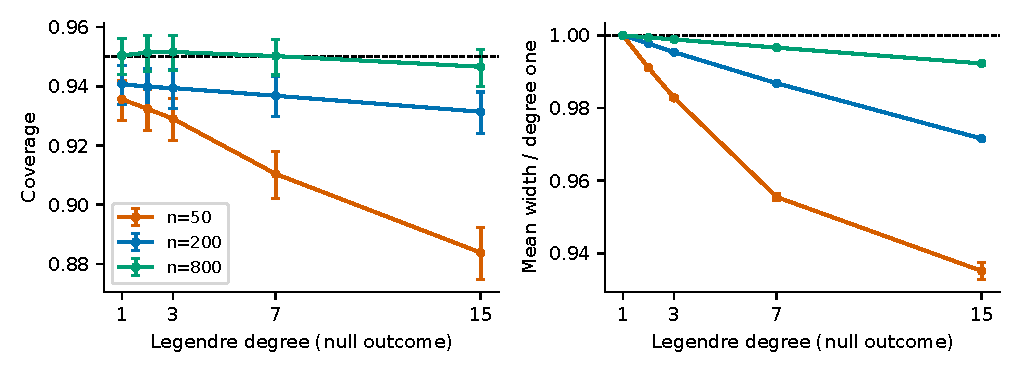
\includegraphics[width=.87\linewidth]{generated/ablation.pdf}
 \caption{Degree stress test on uninformative scores. Five thousand repetitions per point. Left: coverage with Wilson 95\% Monte Carlo intervals; right: width relative to degree one with paired errors. A shorter interval without nominal coverage is a failure.}
 \label{fig:ablation}
\end{figure}

\subsection{What survives a finite-sample guarantee?}
\begin{table}[t]
 \caption{Finite-sample-valid intervals. Baseline is EB-label for continuous outcomes and the exact binomial interval for binary outcomes. At $n=800$ there are 5,000 repetitions; at $12,800$ there are 3,000; $N=10n$. Width bars are 95\% Monte Carlo errors. Coverage is empirical, while the coverage lower bound follows from Theorem~\ref{thm:finite}. Full Wilson intervals include the nonzero uncertainty when coverage is 100\%.}
 \label{tab:finite}\centering
 \resizebox{\linewidth}{!}{\small
\begin{tabular}{llrrrr}
\toprule
Law & $n$ & Baseline width & EB-split3 width & Cov. (\%) & Width ratio \\
\midrule
Quadratic, continuous & 800 & 0.07565 $\pm$ 0.00003 & 0.09611 $\pm$ 0.00001 & 100.00 $\pm$ 0.00 & 1.2704 $\pm$ 0.0004 \\
Quadratic, continuous & 12800 & 0.01411 $\pm$ 2.1e-06 & 0.01012 $\pm$ 5.1e-07 & 100.00 $\pm$ 0.00 & 0.7169 $\pm$ 0.0001 \\
Uninformative & 800 & 0.07039 $\pm$ 1.7e-06 & 0.20530 $\pm$ 0.00007 & 100.00 $\pm$ 0.00 & 2.917 $\pm$ 0.001 \\
Uninformative & 12800 & 0.01740 $\pm$ 3.3e-08 & 0.03639 $\pm$ 4.4e-06 & 99.97 $\pm$ 0.07 & 2.0914 $\pm$ 0.0003 \\
Rare event & 800 & 0.01110 $\pm$ 0.00007 & 0.05073 $\pm$ 0.00015 & 100.00 $\pm$ 0.00 & 4.569 $\pm$ 0.016 \\
Rare event & 12800 & 0.00252 $\pm$ 0.00001 & 0.00904 $\pm$ 0.00002 & 100.00 $\pm$ 0.00 & 3.581 $\pm$ 0.004 \\
\bottomrule
\end{tabular}
}
\end{table}
The strict-coverage comparison changes the practical conclusion (Table~\ref{tab:finite}). In the continuous quadratic example at $n=800$, EB-split3 is wider than EB-label by the ratio \FiniteSmallRatio{}. At $n=3,200$, the reduction is \FiniteMidReduction\%; at $n=12,800$, the ratio is \FiniteLargeRatio{}: a \FiniteReduction\% reduction with coverage \FiniteLargeCoverage{}. This demonstrates a shorter interval with an actual finite-sample coverage theorem under fixed inputs. The large label count is a limitation, not an extra resource granted to the proposed method: every comparator in that row gets the same labels. EB-split3 remains much wider than an oracle-normal interval, so this result does not establish optimal finite-sample width.

In the uninformative and rare-event binary laws, exact binomial intervals are much narrower than the split bound. On the three real artifacts, even at $n=800$ the strict split bound is wider than the existing valid label-only methods; the available results do not support practical strict-coverage improvement there. An unreported reduction against only EB-raw would be a weak comparison because ignoring the predictor already helps. Finally, the unlabeled-size check follows the $\rho$ factor in the headroom formula: nonlinear gains increase when unlabeled observations are plentiful, but vanish in the no-information example. Figure~\ref{fig:ratio} in the appendix reports coverage as well as width.

\section{Discussion and limitations}
\label{sec:limits}
With fixed observations and a fixed predictor, inference can still exploit nonlinear score information that scalar power tuning discards. The achievable first-order gain is limited by conditional noise and by estimating the score distribution. When the conditional mean is already affine, the regular score-only bound leaves no extra first-order gain. A low-dimensional dictionary can approximate a useful nonlinearity; it cannot guarantee improvement, and flexible empirical fitting can make intervals misleadingly small.

Our strongest numerical reductions concern asymptotic intervals in deliberately favorable synthetic laws. Strict finite-sample improvement is demonstrated only against specified bounded-outcome baselines in a large-label continuous example. We do not show an improvement over the best possible finite-sample procedure. Exact binomial intervals decisively outperform our strict bound on binary no-information examples. We do not recommend replacing exact binary intervals with the split construction merely to use a predictor.

The real-data study conditions on empirical artifact distributions, and does not validate the original model's external training independence, annotations, spatial dependence, or deployment sampling. The theory needs representative IID samples from the same score law. Covariate shift, informative label selection, clustered observations, label noise relative to a scientific gold standard, or a predictor trained on the inference labels invalidate this unmodified analysis. We do not repair those violations. We study only means, bounded outcomes for exact guarantees, small prespecified dictionaries, and fixed folds. Gaussian asymptotics are pointwise rather than uniform near rare-event or degenerate distributions. Further transformations, extra recorded features, and other interval constructions might improve the small headroom found here; the cubic real-data result is not an impossibility theorem.

The reproducibility package contains all \TotalRepetitions{} reported repetitions in \TotalCells{} conditions, including negative results, exact commands, environment versions, and access/failure logs. CPU resources and measured runtimes are in Appendix~\ref{app:reproduce}. No human-subject data were collected. A practical benefit is more precise inference without additional annotation; a practical harm is false certainty if a narrow interval's assumptions or empirical coverage are ignored. Coverage failures are therefore first-class outputs. The finite-sample bounds are often conservative; equal nominal coverage does not imply equal achieved coverage. Existing artifact licenses are incompletely specified; code licensing is not treated as permission to relicense the data. This report was designed, implemented, and written by an autonomous language-model agent; the artifact enables independent review of its numerical and mathematical claims, which have not undergone human peer review.

\clearpage
\bibliographystyle{plainnat}
\bibliography{references}

\clearpage
\appendix
\section{Proofs and precise scope}
\label{app:proofs}
\subsection{Projection calculation and nonlinear headroom}
Let all random variables be centered when computing covariance. Expand Equation~\eqref{eq:est}:
\begin{equation}
 n V(b)=\Var Y-2b^\top c+(1+n/N)b^\top\Sigma b.
 \label{eq:expand}
\end{equation}
Since $1+n/N=1/\rho$, square completion gives Equations~\eqref{eq:opt}--\eqref{eq:regret}. The centered projection of $m$ onto the dictionary is $c^\top\Sigma^{-1}(\phi-\E\phi)$ because $\Cov(\phi,Y)=\Cov(\phi,m)$. Its squared norm is $c^\top\Sigma^{-1}c$. For nested subspaces, orthogonality makes the difference in squared projection norms the squared norm of the added component. This proves the nested-gain statement.

For an arbitrary square-integrable control $h(S)$, $\Cov(Y,h)=\Cov(m,h)$. Complete the square in the Hilbert space of centered functions of $S$: the optimum is $h^*(S)=\rho\{m(S)-\mu\}$, up to an irrelevant constant, and $n V_S^*=\Var Y-\rho\Var m$. Apply the variance decomposition $\Var Y=\sigma_\epsilon^2+\sigma_m^2$ and $1-\rho=n/(n+N)$ to get Equation~\eqref{eq:headroom}. Its last difference is the squared residual after affine projection. With a singular dictionary, perform these calculations on a fixed orthonormal basis for its nonconstant span. The pseudoinverse gives the same estimator whenever this span has fixed rank; this is the two-valued-score case in our implementation. We do not assert stable pseudoinverse behavior for an arbitrarily changing numerical rank.

\subsection{Influence-function lower bound}
For clarity, the regularity class in Proposition~\ref{prop:lower} consists of centered, finite-variance influence functions $a(Y,S)$ and $b(S)$ in an expansion
\begin{equation}
 \widehat\mu-\mu=\frac1n\sum_{i=1}^n a(Y_i,S_i)+\frac1N\sum_{j=1}^N b(\widetilde S_j)+o_P(n^{-1/2}),
 \label{eq:if}
\end{equation}
regular along all bounded, mean-zero likelihood-score paths $h(Y,S)$ of the unrestricted joint distribution. Such a path induces marginal score $\E[h\mid S]$ in the unlabeled sample. Differentiating the mean functional and the regular expansion gives
\begin{equation}
 \E[a h]+\E[b\E(h\mid S)]=\E[(Y-\mu)h]\quad\text{for every such }h.
 \label{eq:tangent}
\end{equation}
By iterated expectations and density of bounded centered scores in $L^2_0(P)$, $a(Y,S)+b(S)=Y-\mu$ almost surely; both sides have zero expectation. The first-order variance of Equation~\eqref{eq:if} is therefore
\begin{align}
 \frac{\E[(Y-\mu-b(S))^2]}n+\frac{\E[b(S)^2]}N
 &=\frac{\sigma_\epsilon^2}n+
   \frac{\E[(m-\mu-b(S))^2]}n+\frac{\E[b(S)^2]}N\\
 &=V_S^*+(n^{-1}+N^{-1})\E[(b-\rho(m-\mu))^2].
 \label{eq:ifbound}
\end{align}
This proves the claimed lower bound and its equality condition. The argument is local and first-order. It does not exclude superefficiency at isolated distributions or shorter intervals with nonstandard coverage/length tradeoffs, and it is not a lower bound over arbitrary finite-sample confidence sets. Statements about oracle interval ratios in this paper concern normal, symmetric, first-order intervals only.

\subsection{Consistency and Wald coverage}
Let $d$ be fixed. Under the fourth-moment and nonsingularity assumptions of Proposition~\ref{prop:wald}, sample covariance matrices and cross-covariances converge to their population values. Since $\rho$ converges to a constant, $\widehat b-b_d^*=o_P(1)$. Meanwhile, $\bar\phi_U-\bar\phi_L=O_P(n^{-1/2})$ when $n/N\to r\in(0,\infty)$. Thus
\begin{equation}
 \widehat\mu_{\widehat b}-\widehat\mu_{b_d^*}
 =(\widehat b-b_d^*)^\top(\bar\phi_U-\bar\phi_L)=o_P(n^{-1/2}).
 \label{eq:remainder}
\end{equation}
The two independent sample means for fixed $b_d^*$ satisfy the multivariate central limit theorem; with positive limiting variance, the standardized oracle estimator tends to a standard normal distribution. Continuous mapping and the moment laws imply consistency of the plug-in variance, so Slutsky's theorem yields the Wald coverage statement.

In CF3, each fixed fold's training OLS slope converges to $\Sigma^{-1}c$, whether or not the conditional mean is cubic. Multiplying by $\rho$ therefore gives $b_d^*+o_P(1)$. Fold proportions are fixed and positive, and each difference $\bar\phi_U-\bar\phi_{L_k}$ is $O_P(n^{-1/2})$. Summing the finitely many products proves asymptotic equivalence to the same oracle estimator. Within-fold sample residual variances consistently estimate $\Var(Y-b_d^{*\top}\phi)$. The average slope converges to $b_d^*$, so Equation~\eqref{eq:cfvar} consistently estimates the oracle two-sample variance. All reported fold sizes are equal. With unequal fold sizes, Equation~\eqref{eq:cf} and the average coefficient must instead use weights $|L_k|/n$, which the supplied implementation does.

These arguments explain fixed-dimensional asymptotic validity, but do not bound remainders at a particular $n$ or for growing $d$. In particular, a small oracle variance can make an $o_P(n^{-1/2})$ term practically important. Neither the degree stress test nor rare-event failures contradict this pointwise theorem.

\subsection{Finite-sample coverage and pilot cost}
For a variable $Z\in[a,a+R]$, apply \citet[Theorem~4]{bernstein} to $(Z-a)/R$ with failure probability $\delta/2$ and to $1-(Z-a)/R$ with the same probability. Scaling back gives Equation~\eqref{eq:eb} simultaneously for both signs with total error at most $\delta$. The theorem uses the unbiased sample variance, which equals the pairwise-difference definition in that source.

Let $\mathcal P$ be the pilot sigma field. The pilot is chosen by fixed indices before observing data. Conditional on $\mathcal P$, $g$ is fixed, $0\le g\le\rho_\ell$, and the inference pairs and unlabeled scores are independent IID samples from their original laws. The residual lies in $[-\rho_\ell,1]$. Consequently,
\begin{align}
 \Pr\{ |\overline{Y-g}_I-\E(Y-g)|>B_\ell(s_I^2(Y-g),1+\rho_\ell,\alpha/2)\mid\mathcal P\}&\le\alpha/2,\\
 \Pr\{ |\bar g_U-\E g|>B_N(s_U^2(g),\rho_\ell,\alpha/2)\mid\mathcal P\}&\le\alpha/2.
 \label{eq:twobounds}
\end{align}
On the complement of these two failure events, their sum differs from $\mu$ by at most Equation~\eqref{eq:split}. A union bound and expectation over $\mathcal P$ give coverage at least $1-\alpha$. Clipping interval endpoints into $[0,1]$ cannot remove a true parameter in that set. No pilot calibration accuracy, conditional-mean specification, or large-sample approximation is needed.

To derive Equation~\eqref{eq:splitcost}, condition on $\mathcal P$ and expand
\begin{equation}
 \Var(\overline{Y-g}_I+\bar g_U\mid\mathcal P)
 =\frac{\Var(Y-g)}\ell+\frac{\Var g}N.
 \label{eq:pilotvar}
\end{equation}
The conditional mean is always $\mu$. Square completion with respect to the centered control $g$ gives Equation~\eqref{eq:splitcost}, up to constants in $g$ that do not affect variance. Thus the unconditional estimator variance is the expectation of that expression. Relative to a full-data score oracle, its excess is
\begin{align}
 &\sigma_\epsilon^2(\ell^{-1}-n^{-1})
 +\sigma_m^2\{(\ell+N)^{-1}-(n+N)^{-1}\}\notag\\
 &\qquad +(\ell^{-1}+N^{-1})\E_{\mathcal P}\Var\{g(S)-\rho_\ell m(S)\}.
 \label{eq:costs}
\end{align}
Every term is nonnegative. To outperform a full-data scalar oracle \emph{in point-estimator variance}, the nonlinear headroom in Equation~\eqref{eq:headroom} must exceed these costs. To outperform its confidence-interval width, one must additionally account for the different coverage construction, including the explicit range penalties. This distinction is central to the finite-sample experiment.

The exact binary baseline uses $k=\sum_iY_i$ and endpoints $0$ if $k=0$ (otherwise $\operatorname{Beta}^{-1}_{\alpha/2}(k,n-k+1)$), and $1$ if $k=n$ (otherwise $\operatorname{Beta}^{-1}_{1-\alpha/2}(k+1,n-k)$). Inverting each binomial tail gives tail noncoverage at most $\alpha/2$; summing the two errors gives coverage at least $1-\alpha$. Binary support is known from the law or artifact, not inferred from whether the observed sample happens to contain only zeros and ones. Hoeffding's baseline has half-width $\sqrt{\log(2/\alpha)/(2n)}$ and the same endpoint clipping.

\clearpage
\section{Oracle checks and sample-size sensitivity}
\label{app:oracles}
\begin{table}[h]
 \centering\caption{Oracle width ratios and measured CF3 width at $n=800$, $N=8,000$. All-score ratios are first-order lower bounds under the regularity conditions of Proposition~\ref{prop:lower}, not finite-sample interval bounds. Oracle moments are computed by exact piecewise-polynomial integration in \texttt{experiment.py}; measured widths use the actual repetitions.}
 \resizebox{\linewidth}{!}{\small
\begin{tabular}{lrrrr}
\toprule
Law & Cubic / linear oracle & All-score / linear bound & Cubic oracle width & CF3 width \\
\midrule
Linear, continuous & 1.000 & 1.000 & 0.00994 & 0.00994 $\pm$ 1.4e-06 \\
Quadratic, continuous & 0.309 & 0.309 & 0.01025 & 0.01025 $\pm$ 1.7e-06 \\
Linear, binary & 1.000 & 1.000 & 0.06019 & 0.06026 $\pm$ 0.00003 \\
Quadratic, binary & 0.844 & 0.844 & 0.05579 & 0.05590 $\pm$ 0.00003 \\
Threshold, binary & 0.883 & 0.724 & 0.04241 & 0.04246 $\pm$ 0.00004 \\
Uninformative & 1.000 & 1.000 & 0.06930 & 0.06944 $\pm$ 0.00001 \\
Two-valued score & 1.000 & 1.000 & 0.04481 & 0.04482 $\pm$ 0.00005 \\
Rare event & 1.000 & 1.000 & 0.00978 & 0.00942 $\pm$ 0.00007 \\
\bottomrule
\end{tabular}
}
\end{table}
\begin{figure}[h]
 \centering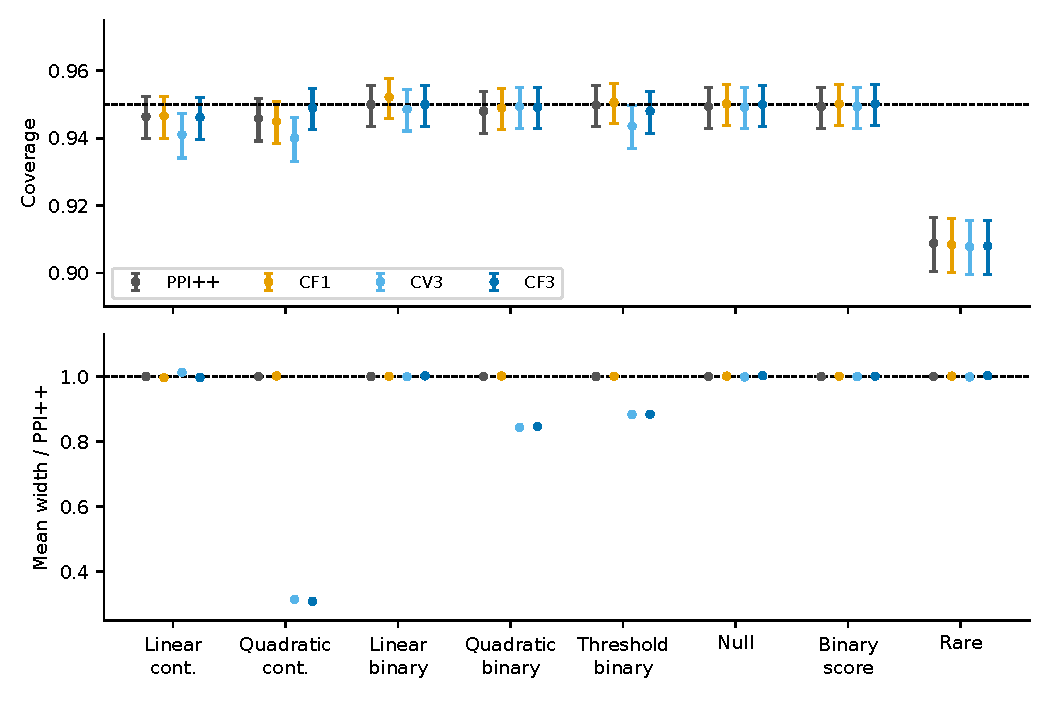
\includegraphics[width=.93\linewidth]{generated/synthetic.pdf}
 \caption{Main synthetic comparison. Five thousand repetitions per point; coverage bars are Wilson 95\% intervals, and width-ratio bars are paired delta-method 95\% errors. The rare-event failure remains visible. CV3's extra narrowing can be accompanied by undercoverage.}
\end{figure}
\begin{figure}[h]
 \centering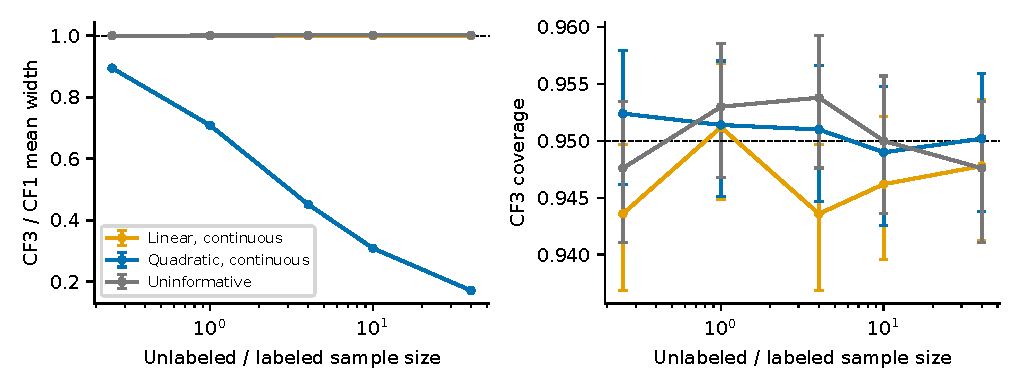
\includegraphics[width=.96\linewidth]{generated/ratio.pdf}
 \caption{Unlabeled-size sensitivity with $n=800$ and 5,000 repetitions per point. Width ratios compare CF3 against CF1, avoiding changes in the scalar fitting algorithm. Coverage bars are Wilson intervals.}
 \label{fig:ratio}
\end{figure}

\clearpage
\section{Prediction artifacts and data provenance}
\label{app:artifacts}
\begin{table}[h]
 \centering\caption{Full artifacts define the empirical evaluation populations. The projection ratio is computed using artifact labels solely as an oracle diagnostic. The interval procedures receive only their sampled labeled pairs and sampled unlabeled scores.}
 \resizebox{\linewidth}{!}{\small
\begin{tabular}{lrrr}
\toprule
Artifact & Records & Empirical target & Cubic/linear oracle width \\
\midrule
Galaxies & 16743 & 0.259273 & 1.0000 \\
Forest & 1596 & 0.151629 & 0.9961 \\
Protein disorder & 10802 & 0.177375 & 0.9987 \\
\bottomrule
\end{tabular}
}
\end{table}
The artifact version is pinned to the Google Drive identifiers in the \texttt{v0.2.3} loader at \url{https://github.com/aangelopoulos/ppi_py/tree/v0.2.3}. The galaxies notebook attributes labels to Galaxy Zoo~2, based on Sloan Digital Sky Survey images, and describes the spiral-arm prevalence target. The forest notebook attributes field labels to Bullock and colleagues and tree-cover predictions to Sexton and colleagues. The alphafold notebook attributes disorder-related labels to Iakoucheva and colleagues and predicted structures/disorder processing to Jumper and colleagues and Bludau and colleagues. These attributions were read in the version-pinned notebooks, which are retained in \texttt{literature/}; the original source studies were not used for additional empirical claims or added to the reference list without being read. Our alphafold target is mean disorder prevalence, rather than the notebook's modification odds ratio.

The reference code is MIT licensed, with its LICENSE retained. No independent license for the downloaded NPZ files is supplied in the repository materials checked here. We record that uncertainty rather than assign them the code license. Download instructions, source identifiers, shapes, checksums, and access dates are in the artifact. No new human annotations, personally identifying records, or new model checkpoints are released. Files in the task workspace are research inputs; downstream redistribution should resolve the source data terms independently.

Sampling with replacement can select the same source row more than once, including on both sides of the labeled/unlabeled split. The \emph{indices are independent draws}, so the random variables are independent under the specified empirical-distribution experiment, despite coincident row values. This is different from pretending that a without-replacement partition is an IID superpopulation sample, and different from obtaining new annotations for duplicated records. It estimates resampling performance on the artifact distribution, not the number of unique physical items a scientific study would annotate.

\section{Additional finite-sample results}
\label{app:finite}
Figure~\ref{fig:finite} and the following table include intermediate sample sizes and every strict-coverage comparator. ``Baseline'' in the figure means EB-label for the continuous law and exact binomial for the binary laws. Pointwise Wilson intervals should be used to interpret empirical coverage equal to one: it is not proof of population coverage exactly one.
\begin{figure}[h]
 \centering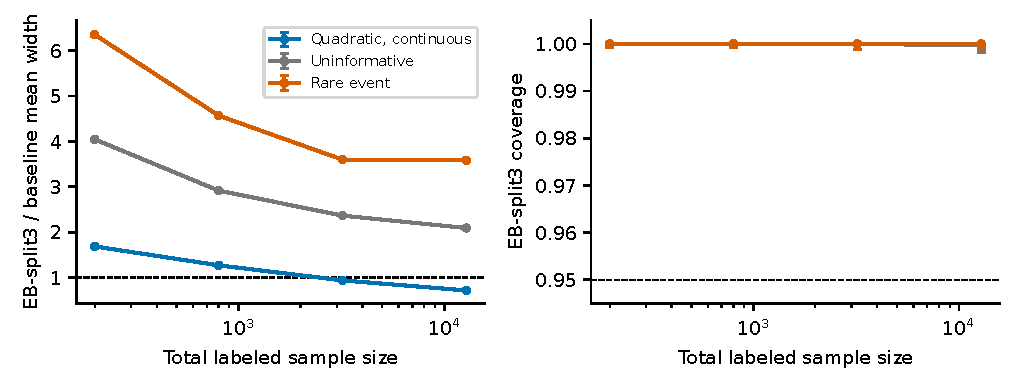
\includegraphics[width=.96\linewidth]{generated/finite.pdf}
 \caption{Strict-coverage tradeoff as the label count changes; $N=10n$. All methods within a point have identical inputs. Error bars are Wilson intervals for coverage and paired delta-method errors for ratios.}
 \label{fig:finite}
\end{figure}
\begingroup
\scriptsize
\begin{longtable}{lllrrr}
\caption{All finite-sample comparators; widths with 95\% Monte Carlo errors, coverage with Wilson 95\% intervals, and paired width ratios.}\\
\toprule
Law & $n$ & Method & Width & Coverage (\%) & Width / EB-label \\
\midrule
\endfirsthead
\toprule
Law & $n$ & Method & Width & Coverage (\%) & Width / EB-label \\
\midrule
\endhead
 &  & Hoeffding & 0.19206 $\pm$ 0.00000 & 100.00 [99.92, 100.00] & 0.9473 $\pm$ 0.0005 \\
Quadratic, continuous & 200 & EB-label & 0.20275 $\pm$ 0.00011 & 100.00 [99.92, 100.00] & 1.000 \\
 &  & EB-raw & 0.45960 $\pm$ 0.00025 & 100.00 [99.92, 100.00] & 2.267 $\pm$ 0.001 \\
 &  & EB-split1 & 0.42551 $\pm$ 0.00025 & 100.00 [99.92, 100.00] & 2.099 $\pm$ 0.001 \\
 &  & EB-split3 & 0.34196 $\pm$ 0.00003 & 100.00 [99.92, 100.00] & 1.687 $\pm$ 0.001 \\
 &  & Hoeffding & 0.09603 $\pm$ 0.00000 & 100.00 [99.92, 100.00] & 1.2694 $\pm$ 0.0004 \\
Quadratic, continuous & 800 & EB-label & 0.07565 $\pm$ 0.00003 & 99.98 [99.89, 100.00] & 1.000 \\
 &  & EB-raw & 0.16722 $\pm$ 0.00006 & 100.00 [99.92, 100.00] & 2.210 $\pm$ 0.001 \\
 &  & EB-split1 & 0.13587 $\pm$ 0.00005 & 100.00 [99.92, 100.00] & 1.796 $\pm$ 0.001 \\
 &  & EB-split3 & 0.09611 $\pm$ 0.00001 & 100.00 [99.92, 100.00] & 1.2704 $\pm$ 0.0004 \\
 &  & Hoeffding & 0.04802 $\pm$ 0.00000 & 100.00 [99.87, 100.00] & 1.5279 $\pm$ 0.0004 \\
Quadratic, continuous & 3200 & EB-label & 0.03143 $\pm$ 0.00001 & 99.97 [99.81, 99.99] & 1.000 \\
 &  & EB-raw & 0.06805 $\pm$ 0.00002 & 100.00 [99.87, 100.00] & 2.165 $\pm$ 0.001 \\
 &  & EB-split1 & 0.04897 $\pm$ 0.00002 & 100.00 [99.87, 100.00] & 1.5583 $\pm$ 0.0004 \\
 &  & EB-split3 & 0.02950 $\pm$ 2.0e-06 & 100.00 [99.87, 100.00] & 0.9386 $\pm$ 0.0002 \\
 &  & Hoeffding & 0.02401 $\pm$ 0.00000 & 100.00 [99.87, 100.00] & 1.7010 $\pm$ 0.0003 \\
Quadratic, continuous & 12800 & EB-label & 0.01411 $\pm$ 2.1e-06 & 99.93 [99.76, 99.98] & 1.000 \\
 &  & EB-raw & 0.03014 $\pm$ 0.00001 & 100.00 [99.87, 100.00] & 2.1356 $\pm$ 0.0003 \\
 &  & EB-split1 & 0.01977 $\pm$ 3.7e-06 & 100.00 [99.87, 100.00] & 1.4007 $\pm$ 0.0002 \\
 &  & EB-split3 & 0.01012 $\pm$ 5.1e-07 & 100.00 [99.87, 100.00] & 0.7169 $\pm$ 0.0001 \\
 &  & Hoeffding & 0.19206 $\pm$ 0.00000 & 99.44 [99.19, 99.61] & 0.6154 $\pm$ 4.1e-05 \\
 &  & Exact-binomial & 0.14234 $\pm$ 0.00001 & 95.48 [94.87, 96.02] & 0.4561 $\pm$ 1.3e-05 \\
Uninformative & 200 & EB-label & 0.31209 $\pm$ 0.00002 & 100.00 [99.92, 100.00] & 1.000 \\
 &  & EB-raw & 0.55086 $\pm$ 0.00023 & 100.00 [99.92, 100.00] & 1.765 $\pm$ 0.001 \\
 &  & EB-split1 & 0.56099 $\pm$ 0.00029 & 100.00 [99.92, 100.00] & 1.798 $\pm$ 0.001 \\
 &  & EB-split3 & 0.57585 $\pm$ 0.00039 & 100.00 [99.92, 100.00] & 1.845 $\pm$ 0.001 \\
 &  & Hoeffding & 0.09603 $\pm$ 0.00000 & 99.28 [99.00, 99.48] & 0.7372 $\pm$ 1.4e-05 \\
 &  & Exact-binomial & 0.07039 $\pm$ 1.7e-06 & 95.70 [95.10, 96.23] & 0.5404 $\pm$ 2.3e-06 \\
Uninformative & 800 & EB-label & 0.13026 $\pm$ 2.6e-06 & 99.96 [99.85, 99.99] & 1.000 \\
 &  & EB-raw & 0.21290 $\pm$ 0.00006 & 100.00 [99.92, 100.00] & 1.6344 $\pm$ 0.0004 \\
 &  & EB-split1 & 0.20247 $\pm$ 0.00006 & 100.00 [99.92, 100.00] & 1.5543 $\pm$ 0.0004 \\
 &  & EB-split3 & 0.20530 $\pm$ 0.00007 & 100.00 [99.92, 100.00] & 1.576 $\pm$ 0.001 \\
 &  & Hoeffding & 0.04802 $\pm$ 0.00000 & 99.53 [99.22, 99.72] & 0.8176 $\pm$ 5.6e-06 \\
 &  & Exact-binomial & 0.03494 $\pm$ 2.6e-07 & 95.10 [94.27, 95.82] & 0.5950 $\pm$ 4.5e-07 \\
Uninformative & 3200 & EB-label & 0.05873 $\pm$ 4.0e-07 & 99.97 [99.81, 99.99] & 1.000 \\
 &  & EB-raw & 0.09087 $\pm$ 0.00002 & 100.00 [99.87, 100.00] & 1.5474 $\pm$ 0.0003 \\
 &  & EB-split1 & 0.08203 $\pm$ 0.00002 & 100.00 [99.87, 100.00] & 1.3969 $\pm$ 0.0003 \\
 &  & EB-split3 & 0.08266 $\pm$ 0.00002 & 100.00 [99.87, 100.00] & 1.4075 $\pm$ 0.0003 \\
 &  & Hoeffding & 0.02401 $\pm$ 0.00000 & 99.57 [99.26, 99.75] & 0.8647 $\pm$ 1.5e-06 \\
 &  & Exact-binomial & 0.01740 $\pm$ 3.3e-08 & 94.97 [94.13, 95.69] & 0.6267 $\pm$ 6.3e-08 \\
Uninformative & 12800 & EB-label & 0.02776 $\pm$ 5.0e-08 & 99.90 [99.71, 99.97] & 1.000 \\
 &  & EB-raw & 0.04154 $\pm$ 4.6e-06 & 100.00 [99.87, 100.00] & 1.4962 $\pm$ 0.0002 \\
 &  & EB-split1 & 0.03625 $\pm$ 3.8e-06 & 99.97 [99.81, 99.99] & 1.3056 $\pm$ 0.0001 \\
 &  & EB-split3 & 0.03639 $\pm$ 4.4e-06 & 99.97 [99.81, 99.99] & 1.3106 $\pm$ 0.0002 \\
 &  & Hoeffding & 0.10103 $\pm$ 0.00014 & 100.00 [99.92, 100.00] & 1.489 $\pm$ 0.007 \\
 &  & Exact-binomial & 0.02648 $\pm$ 0.00021 & 97.94 [97.51, 98.30] & 0.390 $\pm$ 0.001 \\
Rare event & 200 & EB-label & 0.06783 $\pm$ 0.00039 & 100.00 [99.92, 100.00] & 1.000 \\
 &  & EB-raw & 0.21687 $\pm$ 0.00062 & 100.00 [99.92, 100.00] & 3.197 $\pm$ 0.018 \\
 &  & EB-split1 & 0.16750 $\pm$ 0.00048 & 100.00 [99.92, 100.00] & 2.469 $\pm$ 0.008 \\
 &  & EB-split3 & 0.16821 $\pm$ 0.00049 & 100.00 [99.92, 100.00] & 2.480 $\pm$ 0.008 \\
 &  & Hoeffding & 0.05302 $\pm$ 0.00007 & 100.00 [99.92, 100.00] & 2.129 $\pm$ 0.008 \\
 &  & Exact-binomial & 0.01110 $\pm$ 0.00007 & 95.94 [95.36, 96.45] & 0.4459 $\pm$ 0.0005 \\
Rare event & 800 & EB-label & 0.02490 $\pm$ 0.00012 & 100.00 [99.92, 100.00] & 1.000 \\
 &  & EB-raw & 0.08004 $\pm$ 0.00031 & 100.00 [99.92, 100.00] & 3.214 $\pm$ 0.017 \\
 &  & EB-split1 & 0.05058 $\pm$ 0.00015 & 100.00 [99.92, 100.00] & 2.031 $\pm$ 0.005 \\
 &  & EB-split3 & 0.05073 $\pm$ 0.00015 & 100.00 [99.92, 100.00] & 2.037 $\pm$ 0.005 \\
 &  & Hoeffding & 0.02900 $\pm$ 0.00005 & 100.00 [99.87, 100.00] & 2.449 $\pm$ 0.009 \\
 &  & Exact-binomial & 0.00520 $\pm$ 0.00002 & 95.03 [94.20, 95.75] & 0.4395 $\pm$ 0.0004 \\
Rare event & 3200 & EB-label & 0.01184 $\pm$ 0.00006 & 100.00 [99.87, 100.00] & 1.000 \\
 &  & EB-raw & 0.03451 $\pm$ 0.00020 & 100.00 [99.87, 100.00] & 2.914 $\pm$ 0.020 \\
 &  & EB-split1 & 0.01869 $\pm$ 0.00007 & 100.00 [99.87, 100.00] & 1.579 $\pm$ 0.004 \\
 &  & EB-split3 & 0.01873 $\pm$ 0.00007 & 100.00 [99.87, 100.00] & 1.582 $\pm$ 0.004 \\
 &  & Hoeffding & 0.01701 $\pm$ 0.00002 & 100.00 [99.87, 100.00] & 3.219 $\pm$ 0.001 \\
 &  & Exact-binomial & 0.00252 $\pm$ 0.00001 & 95.23 [94.41, 95.94] & 0.4777 $\pm$ 0.0003 \\
Rare event & 12800 & EB-label & 0.00528 $\pm$ 0.00001 & 100.00 [99.87, 100.00] & 1.000 \\
 &  & EB-raw & 0.01780 $\pm$ 0.00010 & 100.00 [99.87, 100.00] & 3.370 $\pm$ 0.018 \\
 &  & EB-split1 & 0.00902 $\pm$ 0.00001 & 100.00 [99.87, 100.00] & 1.708 $\pm$ 0.001 \\
 &  & EB-split3 & 0.00904 $\pm$ 0.00002 & 100.00 [99.87, 100.00] & 1.711 $\pm$ 0.001 \\
\bottomrule
\end{longtable}
\endgroup


\clearpage
\section{Dictionary degree stress test}
\label{app:ablations}
All degrees in this test use full-sample pooled-moment controls, not CF3. The test is a deliberate stress test of an asymptotic approximation as the dictionary becomes large relative to the labels. Each cell has 5,000 paired repetitions, independent from the main suite through separate deterministic seeds. Width reduction without coverage is not counted as a success. Table errors are 95\% Monte Carlo errors; coverage uses Wilson intervals.
\begingroup
\scriptsize
\begin{longtable}{lllrrr}
\caption{All degree stress-test results; 5,000 repetitions per condition. Coverage intervals are Wilson 95\% Monte Carlo intervals.}\\
\toprule
Law & $n$ & Degree & Width & Coverage (\%) & Width / degree one \\
\midrule
\endfirsthead
\toprule
Law & $n$ & Degree & Width & Coverage (\%) & Width / degree one \\
\midrule
\endhead
Linear, continuous & 50 & 1 & 0.04192 $\pm$ 0.00009 & 94.46 [93.79, 95.06] & 1.000 \\
 &  & 2 & 0.04565 $\pm$ 0.00017 & 92.06 [91.28, 92.78] & 1.089 $\pm$ 0.003 \\
 &  & 3 & 0.04900 $\pm$ 0.00027 & 91.02 [90.20, 91.78] & 1.169 $\pm$ 0.005 \\
 &  & 7 & 0.06349 $\pm$ 0.00061 & 89.30 [88.41, 90.13] & 1.514 $\pm$ 0.014 \\
 &  & 15 & 0.09510 $\pm$ 0.00122 & 90.66 [89.82, 91.44] & 2.269 $\pm$ 0.028 \\
Linear, continuous & 200 & 1 & 0.02015 $\pm$ 0.00001 & 94.62 [93.96, 95.21] & 1.000 \\
 &  & 2 & 0.02066 $\pm$ 0.00002 & 93.76 [93.06, 94.40] & 1.026 $\pm$ 0.001 \\
 &  & 3 & 0.02114 $\pm$ 0.00003 & 93.12 [92.38, 93.79] & 1.049 $\pm$ 0.001 \\
 &  & 7 & 0.02308 $\pm$ 0.00007 & 91.58 [90.78, 92.32] & 1.145 $\pm$ 0.003 \\
 &  & 15 & 0.02700 $\pm$ 0.00014 & 89.04 [88.14, 89.88] & 1.340 $\pm$ 0.007 \\
Linear, continuous & 800 & 1 & 0.00998 $\pm$ 2.0e-06 & 94.94 [94.30, 95.51] & 1.000 \\
 &  & 2 & 0.01004 $\pm$ 3.3e-06 & 94.88 [94.23, 95.46] & 1.0066 $\pm$ 0.0003 \\
 &  & 3 & 0.01011 $\pm$ 4.5e-06 & 94.80 [94.15, 95.38] & 1.0130 $\pm$ 0.0004 \\
 &  & 7 & 0.01036 $\pm$ 0.00001 & 93.52 [92.80, 94.17] & 1.038 $\pm$ 0.001 \\
 &  & 15 & 0.01087 $\pm$ 0.00001 & 92.54 [91.78, 93.24] & 1.089 $\pm$ 0.001 \\
Quadratic, continuous & 50 & 1 & 0.13005 $\pm$ 0.00030 & 92.76 [92.01, 93.45] & 1.000 \\
 &  & 2 & 0.04777 $\pm$ 0.00019 & 89.88 [89.01, 90.69] & 0.367 $\pm$ 0.002 \\
 &  & 3 & 0.05188 $\pm$ 0.00033 & 87.86 [86.93, 88.74] & 0.399 $\pm$ 0.002 \\
 &  & 7 & 0.06791 $\pm$ 0.00077 & 79.24 [78.09, 80.34] & 0.522 $\pm$ 0.006 \\
 &  & 15 & 0.10377 $\pm$ 0.00155 & 71.46 [70.19, 72.69] & 0.798 $\pm$ 0.011 \\
Quadratic, continuous & 200 & 1 & 0.06603 $\pm$ 0.00007 & 94.16 [93.48, 94.78] & 1.000 \\
 &  & 2 & 0.02143 $\pm$ 0.00003 & 93.64 [92.93, 94.28] & 0.3246 $\pm$ 0.0005 \\
 &  & 3 & 0.02204 $\pm$ 0.00005 & 92.32 [91.55, 93.03] & 0.334 $\pm$ 0.001 \\
 &  & 7 & 0.02439 $\pm$ 0.00010 & 85.88 [84.89, 86.82] & 0.369 $\pm$ 0.001 \\
 &  & 15 & 0.02902 $\pm$ 0.00019 & 72.68 [71.43, 73.90] & 0.440 $\pm$ 0.003 \\
Quadratic, continuous & 800 & 1 & 0.03311 $\pm$ 0.00002 & 94.66 [94.00, 95.25] & 1.000 \\
 &  & 2 & 0.01037 $\pm$ 3.7e-06 & 94.60 [93.94, 95.19] & 0.3132 $\pm$ 0.0002 \\
 &  & 3 & 0.01045 $\pm$ 0.00001 & 93.78 [93.08, 94.42] & 0.3156 $\pm$ 0.0002 \\
 &  & 7 & 0.01075 $\pm$ 0.00001 & 90.76 [89.93, 91.53] & 0.3247 $\pm$ 0.0003 \\
 &  & 15 & 0.01136 $\pm$ 0.00002 & 83.76 [82.71, 84.76] & 0.343 $\pm$ 0.001 \\
Uninformative & 50 & 1 & 0.27463 $\pm$ 0.00015 & 93.56 [92.85, 94.21] & 1.000 \\
 &  & 2 & 0.27218 $\pm$ 0.00018 & 93.24 [92.51, 93.90] & 0.9911 $\pm$ 0.0004 \\
 &  & 3 & 0.26991 $\pm$ 0.00020 & 92.90 [92.15, 93.58] & 0.9828 $\pm$ 0.0005 \\
 &  & 7 & 0.26241 $\pm$ 0.00026 & 91.04 [90.22, 91.80] & 0.955 $\pm$ 0.001 \\
 &  & 15 & 0.25681 $\pm$ 0.00067 & 88.38 [87.46, 89.24] & 0.935 $\pm$ 0.002 \\
Uninformative & 200 & 1 & 0.13827 $\pm$ 0.00002 & 94.08 [93.39, 94.70] & 1.000 \\
 &  & 2 & 0.13795 $\pm$ 0.00002 & 93.98 [93.29, 94.61] & 0.9977 $\pm$ 0.0001 \\
 &  & 3 & 0.13763 $\pm$ 0.00003 & 93.94 [93.24, 94.57] & 0.9954 $\pm$ 0.0001 \\
 &  & 7 & 0.13644 $\pm$ 0.00003 & 93.68 [92.97, 94.32] & 0.9868 $\pm$ 0.0002 \\
 &  & 15 & 0.13433 $\pm$ 0.00005 & 93.14 [92.41, 93.81] & 0.9715 $\pm$ 0.0003 \\
Uninformative & 800 & 1 & 0.06926 $\pm$ 2.3e-06 & 95.04 [94.40, 95.61] & 1.000 \\
 &  & 2 & 0.06922 $\pm$ 2.8e-06 & 95.14 [94.51, 95.70] & 0.9994 $\pm$ 2.3e-05 \\
 &  & 3 & 0.06918 $\pm$ 3.2e-06 & 95.16 [94.53, 95.72] & 0.9989 $\pm$ 3.1e-05 \\
 &  & 7 & 0.06902 $\pm$ 4.4e-06 & 95.02 [94.38, 95.59] & 0.9966 $\pm$ 0.0001 \\
 &  & 15 & 0.06872 $\pm$ 0.00001 & 94.66 [94.00, 95.25] & 0.9923 $\pm$ 0.0001 \\
\bottomrule
\end{longtable}
\endgroup


\clearpage
\section{Full main results}
\label{app:full}
All tables below use $N=10n$ and 5,000 repetitions. Widths show mean $\pm1.96$ standard errors; coverage shows the estimate followed by its Wilson 95\% Monte Carlo interval, in percent. Ratios compare mean widths to unrestricted scalar PPI++ with paired delta-method errors. They are descriptive ratios, including when either procedure under-covers. Exact-binomial rows are present only for known binary outcomes. The clipped PPI++ rows use the reference package's $[0,1]$ coefficient restriction; all methods use the declared unbiased covariance/variance convention. Large Monte Carlo errors or zero mean widths are never silently removed.
\clearpage
\subsection{Linear continuous}
\begin{table}[h]
\centering\caption{Linear continuous, $n=200$, $N=2000$.}
\resizebox{\linewidth}{!}{\small
\begin{tabular}{lrrr}
\toprule
Method & Width & Coverage (\%) & Width / PPI++ \\
\midrule
Classical & 0.06416 $\pm$ 0.00006 & 94.62 [93.96, 95.21] & 3.184 $\pm$ 0.003 \\
PPI & 0.03032 $\pm$ 0.00001 & 95.04 [94.40, 95.61] & 1.504 $\pm$ 0.001 \\
PPI++ & 0.02015 $\pm$ 0.00001 & 94.62 [93.96, 95.21] & 1.000 \\
PPI++clip & 0.02015 $\pm$ 0.00001 & 94.62 [93.96, 95.21] & 1.000 \\
CF1 & 0.01989 $\pm$ 0.00001 & 95.04 [94.40, 95.61] & 0.987 $\pm$ 0.001 \\
CV3 & 0.02116 $\pm$ 0.00004 & 93.14 [92.41, 93.81] & 1.050 $\pm$ 0.002 \\
CF3 & 0.01990 $\pm$ 0.00001 & 94.96 [94.32, 95.53] & 0.987 $\pm$ 0.001 \\
Hoeffding & 0.19206 $\pm$ 0.00000 & 100.00 [99.92, 100.00] & 9.531 $\pm$ 0.006 \\
EB-label & 0.19968 $\pm$ 0.00009 & 100.00 [99.92, 100.00] & 9.908 $\pm$ 0.006 \\
EB-raw & 0.31814 $\pm$ 0.00003 & 100.00 [99.92, 100.00] & 15.787 $\pm$ 0.009 \\
EB-split1 & 0.34059 $\pm$ 0.00002 & 100.00 [99.92, 100.00] & 16.901 $\pm$ 0.010 \\
EB-split3 & 0.34075 $\pm$ 0.00003 & 100.00 [99.92, 100.00] & 16.909 $\pm$ 0.010 \\
\bottomrule
\end{tabular}
}
\end{table}
\begin{table}[h]
\centering\caption{Linear continuous, $n=800$, $N=8000$.}
\resizebox{\linewidth}{!}{\small
\begin{tabular}{lrrr}
\toprule
Method & Width & Coverage (\%) & Width / PPI++ \\
\midrule
Classical & 0.03209 $\pm$ 0.00001 & 95.20 [94.57, 95.76] & 3.217 $\pm$ 0.001 \\
PPI & 0.01516 $\pm$ 2.6e-06 & 94.04 [93.35, 94.66] & 1.5194 $\pm$ 0.0003 \\
PPI++ & 0.00998 $\pm$ 2.0e-06 & 94.64 [93.98, 95.23] & 1.000 \\
PPI++clip & 0.00998 $\pm$ 2.0e-06 & 94.64 [93.98, 95.23] & 1.000 \\
CF1 & 0.00994 $\pm$ 1.4e-06 & 94.66 [94.00, 95.25] & 0.9966 $\pm$ 0.0001 \\
CV3 & 0.01011 $\pm$ 4.7e-06 & 94.10 [93.41, 94.72] & 1.0133 $\pm$ 0.0004 \\
CF3 & 0.00994 $\pm$ 1.4e-06 & 94.62 [93.96, 95.21] & 0.9967 $\pm$ 0.0001 \\
Hoeffding & 0.09603 $\pm$ 0.00000 & 100.00 [99.92, 100.00] & 9.625 $\pm$ 0.002 \\
EB-label & 0.07407 $\pm$ 0.00002 & 100.00 [99.92, 100.00] & 7.424 $\pm$ 0.002 \\
EB-raw & 0.09639 $\pm$ 0.00001 & 100.00 [99.92, 100.00] & 9.660 $\pm$ 0.002 \\
EB-split1 & 0.09550 $\pm$ 0.00001 & 100.00 [99.92, 100.00] & 9.571 $\pm$ 0.002 \\
EB-split3 & 0.09551 $\pm$ 0.00001 & 100.00 [99.92, 100.00] & 9.573 $\pm$ 0.002 \\
\bottomrule
\end{tabular}
}
\end{table}
\clearpage
\subsection{Quadratic continuous}
\begin{table}[h]
\centering\caption{Quadratic continuous, $n=200$, $N=2000$.}
\resizebox{\linewidth}{!}{\small
\begin{tabular}{lrrr}
\toprule
Method & Width & Coverage (\%) & Width / PPI++ \\
\midrule
Classical & 0.06620 $\pm$ 0.00007 & 95.14 [94.51, 95.70] & 1.0036 $\pm$ 0.0001 \\
PPI & 0.10677 $\pm$ 0.00015 & 94.58 [93.92, 95.17] & 1.619 $\pm$ 0.002 \\
PPI++ & 0.06596 $\pm$ 0.00007 & 94.92 [94.28, 95.49] & 1.000 \\
PPI++clip & 0.06608 $\pm$ 0.00007 & 95.06 [94.42, 95.63] & 1.0017 $\pm$ 0.0001 \\
CF1 & 0.06651 $\pm$ 0.00007 & 95.18 [94.55, 95.74] & 1.0083 $\pm$ 0.0003 \\
CV3 & 0.02201 $\pm$ 0.00004 & 91.68 [90.88, 92.41] & 0.334 $\pm$ 0.001 \\
CF3 & 0.02051 $\pm$ 0.00001 & 95.06 [94.42, 95.63] & 0.3109 $\pm$ 0.0003 \\
Hoeffding & 0.19206 $\pm$ 0.00000 & 100.00 [99.92, 100.00] & 2.912 $\pm$ 0.003 \\
EB-label & 0.20275 $\pm$ 0.00011 & 100.00 [99.92, 100.00] & 3.074 $\pm$ 0.002 \\
EB-raw & 0.45960 $\pm$ 0.00025 & 100.00 [99.92, 100.00] & 6.967 $\pm$ 0.007 \\
EB-split1 & 0.42551 $\pm$ 0.00025 & 100.00 [99.92, 100.00] & 6.451 $\pm$ 0.006 \\
EB-split3 & 0.34196 $\pm$ 0.00003 & 100.00 [99.92, 100.00] & 5.184 $\pm$ 0.006 \\
\bottomrule
\end{tabular}
}
\end{table}
\begin{table}[h]
\centering\caption{Quadratic continuous, $n=800$, $N=8000$.}
\resizebox{\linewidth}{!}{\small
\begin{tabular}{lrrr}
\toprule
Method & Width & Coverage (\%) & Width / PPI++ \\
\midrule
Classical & 0.03314 $\pm$ 0.00002 & 94.60 [93.94, 95.19] & 1.0009 $\pm$ 3.6e-05 \\
PPI & 0.05345 $\pm$ 0.00004 & 95.02 [94.38, 95.59] & 1.614 $\pm$ 0.001 \\
PPI++ & 0.03311 $\pm$ 0.00002 & 94.58 [93.92, 95.17] & 1.000 \\
PPI++clip & 0.03313 $\pm$ 0.00002 & 94.64 [93.98, 95.23] & 1.0004 $\pm$ 2.8e-05 \\
CF1 & 0.03318 $\pm$ 0.00002 & 94.50 [93.83, 95.10] & 1.0020 $\pm$ 0.0001 \\
CV3 & 0.01045 $\pm$ 0.00001 & 94.00 [93.31, 94.63] & 0.3155 $\pm$ 0.0002 \\
CF3 & 0.01025 $\pm$ 1.7e-06 & 94.90 [94.25, 95.48] & 0.3096 $\pm$ 0.0002 \\
Hoeffding & 0.09603 $\pm$ 0.00000 & 100.00 [99.92, 100.00] & 2.900 $\pm$ 0.002 \\
EB-label & 0.07565 $\pm$ 0.00003 & 99.98 [99.89, 100.00] & 2.2848 $\pm$ 0.0004 \\
EB-raw & 0.16722 $\pm$ 0.00006 & 100.00 [99.92, 100.00] & 5.050 $\pm$ 0.002 \\
EB-split1 & 0.13587 $\pm$ 0.00005 & 100.00 [99.92, 100.00] & 4.103 $\pm$ 0.002 \\
EB-split3 & 0.09611 $\pm$ 0.00001 & 100.00 [99.92, 100.00] & 2.903 $\pm$ 0.001 \\
\bottomrule
\end{tabular}
}
\end{table}
\clearpage
\subsection{Linear binary}
\begin{table}[h]
\centering\caption{Linear binary, $n=200$, $N=2000$.}
\resizebox{\linewidth}{!}{\small
\begin{tabular}{lrrr}
\toprule
Method & Width & Coverage (\%) & Width / PPI++ \\
\midrule
Classical & 0.13858 $\pm$ 0.00001 & 94.36 [93.69, 94.97] & 1.154 $\pm$ 0.001 \\
PPI & 0.12115 $\pm$ 0.00013 & 94.80 [94.15, 95.38] & 1.0088 $\pm$ 0.0002 \\
PPI++ & 0.12009 $\pm$ 0.00011 & 94.52 [93.85, 95.12] & 1.000 \\
PPI++clip & 0.12009 $\pm$ 0.00011 & 94.50 [93.83, 95.10] & 1.0000 $\pm$ 8.0e-06 \\
CF1 & 0.12044 $\pm$ 0.00012 & 94.78 [94.13, 95.36] & 1.0029 $\pm$ 0.0002 \\
CV3 & 0.11990 $\pm$ 0.00011 & 94.34 [93.66, 94.95] & 0.9984 $\pm$ 0.0001 \\
CF3 & 0.12097 $\pm$ 0.00012 & 94.70 [94.04, 95.29] & 1.0073 $\pm$ 0.0003 \\
Hoeffding & 0.19206 $\pm$ 0.00000 & 99.38 [99.12, 99.56] & 1.599 $\pm$ 0.002 \\
EB-label & 0.31208 $\pm$ 0.00002 & 100.00 [99.92, 100.00] & 2.599 $\pm$ 0.002 \\
EB-raw & 0.48358 $\pm$ 0.00022 & 100.00 [99.92, 100.00] & 4.027 $\pm$ 0.002 \\
EB-split1 & 0.54830 $\pm$ 0.00028 & 100.00 [99.92, 100.00] & 4.566 $\pm$ 0.004 \\
EB-split3 & 0.55405 $\pm$ 0.00033 & 100.00 [99.92, 100.00] & 4.613 $\pm$ 0.004 \\
Exact-binomial & 0.14233 $\pm$ 0.00001 & 95.86 [95.27, 96.38] & 1.185 $\pm$ 0.001 \\
\bottomrule
\end{tabular}
}
\end{table}
\begin{table}[h]
\centering\caption{Linear binary, $n=800$, $N=8000$.}
\resizebox{\linewidth}{!}{\small
\begin{tabular}{lrrr}
\toprule
Method & Width & Coverage (\%) & Width / PPI++ \\
\midrule
Classical & 0.06929 $\pm$ 1.8e-06 & 94.44 [93.77, 95.04] & 1.152 $\pm$ 0.001 \\
PPI & 0.06063 $\pm$ 0.00003 & 95.10 [94.47, 95.66] & 1.0081 $\pm$ 0.0001 \\
PPI++ & 0.06014 $\pm$ 0.00003 & 95.00 [94.36, 95.57] & 1.000 \\
PPI++clip & 0.06014 $\pm$ 0.00003 & 95.00 [94.36, 95.57] & 1.0000 $\pm$ 3.0e-08 \\
CF1 & 0.06019 $\pm$ 0.00003 & 95.22 [94.59, 95.78] & 1.0008 $\pm$ 0.0001 \\
CV3 & 0.06012 $\pm$ 0.00003 & 94.86 [94.21, 95.44] & 0.9996 $\pm$ 2.9e-05 \\
CF3 & 0.06026 $\pm$ 0.00003 & 95.00 [94.36, 95.57] & 1.0019 $\pm$ 0.0001 \\
Hoeffding & 0.09603 $\pm$ 0.00000 & 99.12 [98.82, 99.34] & 1.597 $\pm$ 0.001 \\
EB-label & 0.13026 $\pm$ 2.7e-06 & 99.98 [99.89, 100.00] & 2.166 $\pm$ 0.001 \\
EB-raw & 0.17920 $\pm$ 0.00006 & 100.00 [99.92, 100.00] & 2.9795 $\pm$ 0.0005 \\
EB-split1 & 0.19907 $\pm$ 0.00007 & 100.00 [99.92, 100.00] & 3.310 $\pm$ 0.001 \\
EB-split3 & 0.19967 $\pm$ 0.00007 & 100.00 [99.92, 100.00] & 3.320 $\pm$ 0.001 \\
Exact-binomial & 0.07039 $\pm$ 1.8e-06 & 95.30 [94.68, 95.85] & 1.170 $\pm$ 0.001 \\
\bottomrule
\end{tabular}
}
\end{table}
\clearpage
\subsection{Quadratic binary}
\begin{table}[h]
\centering\caption{Quadratic binary, $n=200$, $N=2000$.}
\resizebox{\linewidth}{!}{\small
\begin{tabular}{lrrr}
\toprule
Method & Width & Coverage (\%) & Width / PPI++ \\
\midrule
Classical & 0.13216 $\pm$ 0.00008 & 94.46 [93.79, 95.06] & 1.0032 $\pm$ 0.0001 \\
PPI & 0.15649 $\pm$ 0.00018 & 94.92 [94.28, 95.49] & 1.188 $\pm$ 0.001 \\
PPI++ & 0.13174 $\pm$ 0.00009 & 94.60 [93.94, 95.19] & 1.000 \\
PPI++clip & 0.13195 $\pm$ 0.00008 & 94.56 [93.90, 95.16] & 1.0016 $\pm$ 0.0001 \\
CF1 & 0.13260 $\pm$ 0.00009 & 94.66 [94.00, 95.25] & 1.0065 $\pm$ 0.0002 \\
CV3 & 0.11113 $\pm$ 0.00013 & 93.96 [93.27, 94.59] & 0.844 $\pm$ 0.001 \\
CF3 & 0.11233 $\pm$ 0.00014 & 94.98 [94.34, 95.55] & 0.853 $\pm$ 0.001 \\
Hoeffding & 0.19206 $\pm$ 0.00000 & 99.60 [99.38, 99.74] & 1.458 $\pm$ 0.001 \\
EB-label & 0.30238 $\pm$ 0.00013 & 100.00 [99.92, 100.00] & 2.295 $\pm$ 0.001 \\
EB-raw & 0.54187 $\pm$ 0.00031 & 100.00 [99.92, 100.00] & 4.113 $\pm$ 0.003 \\
EB-split1 & 0.55029 $\pm$ 0.00037 & 100.00 [99.92, 100.00] & 4.177 $\pm$ 0.003 \\
EB-split3 & 0.53944 $\pm$ 0.00035 & 100.00 [99.92, 100.00] & 4.095 $\pm$ 0.003 \\
Exact-binomial & 0.13600 $\pm$ 0.00008 & 95.30 [94.68, 95.85] & 1.0324 $\pm$ 0.0001 \\
\bottomrule
\end{tabular}
}
\end{table}
\begin{table}[h]
\centering\caption{Quadratic binary, $n=800$, $N=8000$.}
\resizebox{\linewidth}{!}{\small
\begin{tabular}{lrrr}
\toprule
Method & Width & Coverage (\%) & Width / PPI++ \\
\midrule
Classical & 0.06610 $\pm$ 0.00002 & 94.54 [93.88, 95.14] & 1.0007 $\pm$ 2.9e-05 \\
PPI & 0.07830 $\pm$ 0.00004 & 94.18 [93.50, 94.80] & 1.185 $\pm$ 0.001 \\
PPI++ & 0.06605 $\pm$ 0.00002 & 94.80 [94.15, 95.38] & 1.000 \\
PPI++clip & 0.06608 $\pm$ 0.00002 & 94.62 [93.96, 95.21] & 1.0004 $\pm$ 2.3e-05 \\
CF1 & 0.06617 $\pm$ 0.00002 & 94.90 [94.25, 95.48] & 1.0017 $\pm$ 0.0001 \\
CV3 & 0.05575 $\pm$ 0.00003 & 94.94 [94.30, 95.51] & 0.8440 $\pm$ 0.0005 \\
CF3 & 0.05590 $\pm$ 0.00003 & 94.92 [94.28, 95.49] & 0.8463 $\pm$ 0.0005 \\
Hoeffding & 0.09603 $\pm$ 0.00000 & 99.64 [99.43, 99.77] & 1.4539 $\pm$ 0.0005 \\
EB-label & 0.12544 $\pm$ 0.00003 & 99.98 [99.89, 100.00] & 1.8990 $\pm$ 0.0001 \\
EB-raw & 0.20841 $\pm$ 0.00007 & 100.00 [99.92, 100.00] & 3.155 $\pm$ 0.001 \\
EB-split1 & 0.19693 $\pm$ 0.00008 & 100.00 [99.92, 100.00] & 2.981 $\pm$ 0.001 \\
EB-split3 & 0.19217 $\pm$ 0.00008 & 100.00 [99.92, 100.00] & 2.909 $\pm$ 0.001 \\
Exact-binomial & 0.06721 $\pm$ 0.00002 & 95.38 [94.76, 95.93] & 1.0175 $\pm$ 3.1e-05 \\
\bottomrule
\end{tabular}
}
\end{table}
\clearpage
\subsection{Threshold binary}
\begin{table}[h]
\centering\caption{Threshold binary, $n=200$, $N=2000$.}
\resizebox{\linewidth}{!}{\small
\begin{tabular}{lrrr}
\toprule
Method & Width & Coverage (\%) & Width / PPI++ \\
\midrule
Classical & 0.12912 $\pm$ 0.00010 & 95.20 [94.57, 95.76] & 1.346 $\pm$ 0.002 \\
PPI & 0.09601 $\pm$ 0.00012 & 95.16 [94.53, 95.72] & 1.0009 $\pm$ 0.0001 \\
PPI++ & 0.09593 $\pm$ 0.00013 & 94.90 [94.25, 95.48] & 1.000 \\
PPI++clip & 0.09601 $\pm$ 0.00012 & 94.98 [94.34, 95.55] & 1.0009 $\pm$ 0.0001 \\
CF1 & 0.09619 $\pm$ 0.00013 & 95.22 [94.59, 95.78] & 1.0027 $\pm$ 0.0002 \\
CV3 & 0.08496 $\pm$ 0.00015 & 94.40 [93.73, 95.00] & 0.886 $\pm$ 0.001 \\
CF3 & 0.08527 $\pm$ 0.00016 & 94.94 [94.30, 95.51] & 0.889 $\pm$ 0.001 \\
Hoeffding & 0.19206 $\pm$ 0.00000 & 99.82 [99.66, 99.91] & 2.002 $\pm$ 0.003 \\
EB-label & 0.29779 $\pm$ 0.00015 & 100.00 [99.92, 100.00] & 3.104 $\pm$ 0.004 \\
EB-raw & 0.44155 $\pm$ 0.00021 & 100.00 [99.92, 100.00] & 4.603 $\pm$ 0.004 \\
EB-split1 & 0.49994 $\pm$ 0.00027 & 100.00 [99.92, 100.00] & 5.212 $\pm$ 0.005 \\
EB-split3 & 0.48884 $\pm$ 0.00036 & 100.00 [99.92, 100.00] & 5.096 $\pm$ 0.005 \\
Exact-binomial & 0.13301 $\pm$ 0.00010 & 96.12 [95.55, 96.62] & 1.387 $\pm$ 0.002 \\
\bottomrule
\end{tabular}
}
\end{table}
\begin{table}[h]
\centering\caption{Threshold binary, $n=800$, $N=8000$.}
\resizebox{\linewidth}{!}{\small
\begin{tabular}{lrrr}
\toprule
Method & Width & Coverage (\%) & Width / PPI++ \\
\midrule
Classical & 0.06463 $\pm$ 0.00002 & 95.10 [94.47, 95.66] & 1.346 $\pm$ 0.001 \\
PPI & 0.04805 $\pm$ 0.00003 & 95.08 [94.45, 95.65] & 1.0005 $\pm$ 2.9e-05 \\
PPI++ & 0.04802 $\pm$ 0.00003 & 94.98 [94.34, 95.55] & 1.000 \\
PPI++clip & 0.04805 $\pm$ 0.00003 & 95.06 [94.42, 95.63] & 1.0005 $\pm$ 2.8e-05 \\
CF1 & 0.04806 $\pm$ 0.00003 & 95.06 [94.42, 95.63] & 1.0007 $\pm$ 4.8e-05 \\
CV3 & 0.04242 $\pm$ 0.00004 & 94.36 [93.69, 94.97] & 0.8834 $\pm$ 0.0004 \\
CF3 & 0.04246 $\pm$ 0.00004 & 94.80 [94.15, 95.38] & 0.8841 $\pm$ 0.0004 \\
Hoeffding & 0.09603 $\pm$ 0.00000 & 99.70 [99.51, 99.82] & 2.000 $\pm$ 0.001 \\
EB-label & 0.12321 $\pm$ 0.00004 & 100.00 [99.92, 100.00] & 2.566 $\pm$ 0.002 \\
EB-raw & 0.15815 $\pm$ 0.00005 & 100.00 [99.92, 100.00] & 3.293 $\pm$ 0.001 \\
EB-split1 & 0.17510 $\pm$ 0.00007 & 100.00 [99.92, 100.00] & 3.646 $\pm$ 0.001 \\
EB-split3 & 0.16880 $\pm$ 0.00008 & 100.00 [99.92, 100.00] & 3.515 $\pm$ 0.001 \\
Exact-binomial & 0.06574 $\pm$ 0.00002 & 95.46 [94.85, 96.00] & 1.369 $\pm$ 0.001 \\
\bottomrule
\end{tabular}
}
\end{table}
\clearpage
\subsection{Uninformative binary}
\begin{table}[h]
\centering\caption{Uninformative binary, $n=200$, $N=2000$.}
\resizebox{\linewidth}{!}{\small
\begin{tabular}{lrrr}
\toprule
Method & Width & Coverage (\%) & Width / PPI++ \\
\midrule
Classical & 0.13859 $\pm$ 0.00001 & 94.12 [93.43, 94.74] & 1.0023 $\pm$ 0.0001 \\
PPI & 0.16185 $\pm$ 0.00014 & 94.34 [93.66, 94.95] & 1.171 $\pm$ 0.001 \\
PPI++ & 0.13826 $\pm$ 0.00002 & 94.28 [93.60, 94.89] & 1.000 \\
PPI++clip & 0.13842 $\pm$ 0.00002 & 94.24 [93.56, 94.85] & 1.0011 $\pm$ 0.0001 \\
CF1 & 0.13899 $\pm$ 0.00004 & 94.42 [93.75, 95.02] & 1.0052 $\pm$ 0.0002 \\
CV3 & 0.13764 $\pm$ 0.00002 & 94.24 [93.56, 94.85] & 0.9955 $\pm$ 0.0001 \\
CF3 & 0.13978 $\pm$ 0.00004 & 94.56 [93.90, 95.16] & 1.0109 $\pm$ 0.0003 \\
Hoeffding & 0.19206 $\pm$ 0.00000 & 99.44 [99.19, 99.61] & 1.3891 $\pm$ 0.0002 \\
EB-label & 0.31209 $\pm$ 0.00002 & 100.00 [99.92, 100.00] & 2.2572 $\pm$ 0.0002 \\
EB-raw & 0.55086 $\pm$ 0.00023 & 100.00 [99.92, 100.00] & 3.984 $\pm$ 0.002 \\
EB-split1 & 0.56099 $\pm$ 0.00029 & 100.00 [99.92, 100.00] & 4.057 $\pm$ 0.002 \\
EB-split3 & 0.57585 $\pm$ 0.00039 & 100.00 [99.92, 100.00] & 4.165 $\pm$ 0.003 \\
Exact-binomial & 0.14234 $\pm$ 0.00001 & 95.48 [94.87, 96.02] & 1.0295 $\pm$ 0.0001 \\
\bottomrule
\end{tabular}
}
\end{table}
\begin{table}[h]
\centering\caption{Uninformative binary, $n=800$, $N=8000$.}
\resizebox{\linewidth}{!}{\small
\begin{tabular}{lrrr}
\toprule
Method & Width & Coverage (\%) & Width / PPI++ \\
\midrule
Classical & 0.06930 $\pm$ 1.7e-06 & 94.96 [94.32, 95.53] & 1.0006 $\pm$ 2.2e-05 \\
PPI & 0.08102 $\pm$ 0.00003 & 94.98 [94.34, 95.55] & 1.1699 $\pm$ 0.0005 \\
PPI++ & 0.06926 $\pm$ 2.3e-06 & 94.94 [94.30, 95.51] & 1.000 \\
PPI++clip & 0.06928 $\pm$ 2.0e-06 & 94.92 [94.28, 95.49] & 1.0003 $\pm$ 1.8e-05 \\
CF1 & 0.06935 $\pm$ 4.4e-06 & 95.02 [94.38, 95.59] & 1.0013 $\pm$ 0.0001 \\
CV3 & 0.06918 $\pm$ 3.1e-06 & 94.92 [94.28, 95.49] & 0.9989 $\pm$ 3.2e-05 \\
CF3 & 0.06944 $\pm$ 0.00001 & 95.00 [94.36, 95.57] & 1.0027 $\pm$ 0.0001 \\
Hoeffding & 0.09603 $\pm$ 0.00000 & 99.28 [99.00, 99.48] & 1.3866 $\pm$ 4.6e-05 \\
EB-label & 0.13026 $\pm$ 2.6e-06 & 99.96 [99.85, 99.99] & 1.8808 $\pm$ 4.3e-05 \\
EB-raw & 0.21290 $\pm$ 0.00006 & 100.00 [99.92, 100.00] & 3.074 $\pm$ 0.001 \\
EB-split1 & 0.20247 $\pm$ 0.00006 & 100.00 [99.92, 100.00] & 2.923 $\pm$ 0.001 \\
EB-split3 & 0.20530 $\pm$ 0.00007 & 100.00 [99.92, 100.00] & 2.964 $\pm$ 0.001 \\
Exact-binomial & 0.07039 $\pm$ 1.7e-06 & 95.70 [95.10, 96.23] & 1.0164 $\pm$ 2.3e-05 \\
\bottomrule
\end{tabular}
}
\end{table}
\clearpage
\subsection{Two-valued score}
\begin{table}[h]
\centering\caption{Two-valued score, $n=200$, $N=2000$.}
\resizebox{\linewidth}{!}{\small
\begin{tabular}{lrrr}
\toprule
Method & Width & Coverage (\%) & Width / PPI++ \\
\midrule
Classical & 0.13859 $\pm$ 0.00001 & 94.10 [93.41, 94.72] & 1.553 $\pm$ 0.003 \\
PPI & 0.09768 $\pm$ 0.00023 & 94.72 [94.07, 95.31] & 1.0946 $\pm$ 0.0003 \\
PPI++ & 0.08924 $\pm$ 0.00018 & 94.50 [93.83, 95.10] & 1.000 \\
PPI++clip & 0.08924 $\pm$ 0.00018 & 94.50 [93.83, 95.10] & 1.000 \\
CF1 & 0.08963 $\pm$ 0.00018 & 94.54 [93.88, 95.14] & 1.0044 $\pm$ 0.0002 \\
CV3 & 0.08924 $\pm$ 0.00018 & 94.50 [93.83, 95.10] & 1.000 \\
CF3 & 0.08963 $\pm$ 0.00018 & 94.54 [93.88, 95.14] & 1.0044 $\pm$ 0.0002 \\
Hoeffding & 0.19206 $\pm$ 0.00000 & 99.60 [99.38, 99.74] & 2.152 $\pm$ 0.004 \\
EB-label & 0.31210 $\pm$ 0.00002 & 100.00 [99.92, 100.00] & 3.497 $\pm$ 0.007 \\
EB-raw & 0.46286 $\pm$ 0.00041 & 100.00 [99.92, 100.00] & 5.187 $\pm$ 0.006 \\
EB-split1 & 0.50359 $\pm$ 0.00042 & 100.00 [99.92, 100.00] & 5.643 $\pm$ 0.009 \\
EB-split3 & 0.50359 $\pm$ 0.00042 & 100.00 [99.92, 100.00] & 5.643 $\pm$ 0.009 \\
Exact-binomial & 0.14234 $\pm$ 0.00001 & 95.92 [95.34, 96.43] & 1.595 $\pm$ 0.003 \\
\bottomrule
\end{tabular}
}
\end{table}
\begin{table}[h]
\centering\caption{Two-valued score, $n=800$, $N=8000$.}
\resizebox{\linewidth}{!}{\small
\begin{tabular}{lrrr}
\toprule
Method & Width & Coverage (\%) & Width / PPI++ \\
\midrule
Classical & 0.06930 $\pm$ 1.6e-06 & 95.08 [94.45, 95.65] & 1.548 $\pm$ 0.002 \\
PPI & 0.04897 $\pm$ 0.00006 & 95.06 [94.42, 95.63] & 1.0938 $\pm$ 0.0002 \\
PPI++ & 0.04477 $\pm$ 0.00005 & 94.94 [94.30, 95.51] & 1.000 \\
PPI++clip & 0.04477 $\pm$ 0.00005 & 94.94 [94.30, 95.51] & 1.000 \\
CF1 & 0.04482 $\pm$ 0.00005 & 95.02 [94.38, 95.59] & 1.0011 $\pm$ 4.8e-05 \\
CV3 & 0.04477 $\pm$ 0.00005 & 94.94 [94.30, 95.51] & 1.000 \\
CF3 & 0.04482 $\pm$ 0.00005 & 95.02 [94.38, 95.59] & 1.0011 $\pm$ 4.8e-05 \\
Hoeffding & 0.09603 $\pm$ 0.00000 & 99.48 [99.24, 99.64] & 2.145 $\pm$ 0.002 \\
EB-label & 0.13026 $\pm$ 2.5e-06 & 99.98 [99.89, 100.00] & 2.909 $\pm$ 0.003 \\
EB-raw & 0.16903 $\pm$ 0.00011 & 100.00 [99.92, 100.00] & 3.776 $\pm$ 0.002 \\
EB-split1 & 0.17654 $\pm$ 0.00011 & 100.00 [99.92, 100.00] & 3.943 $\pm$ 0.003 \\
EB-split3 & 0.17654 $\pm$ 0.00011 & 100.00 [99.92, 100.00] & 3.943 $\pm$ 0.003 \\
Exact-binomial & 0.07039 $\pm$ 1.6e-06 & 95.76 [95.17, 96.28] & 1.572 $\pm$ 0.002 \\
\bottomrule
\end{tabular}
}
\end{table}
\clearpage
\subsection{Rare binary}
\begin{table}[h]
\centering\caption{Rare binary, $n=200$, $N=2000$.}
\resizebox{\linewidth}{!}{\small
\begin{tabular}{lrrr}
\toprule
Method & Width & Coverage (\%) & Width / PPI++ \\
\midrule
Classical & 0.01516 $\pm$ 0.00034 & 63.52 [62.18, 64.84] & 1.0023 $\pm$ 0.0001 \\
PPI & 0.08607 $\pm$ 0.00010 & 95.08 [94.45, 95.65] & 5.689 $\pm$ 0.125 \\
PPI++ & 0.01513 $\pm$ 0.00034 & 63.48 [62.14, 64.80] & 1.000 \\
PPI++clip & 0.01515 $\pm$ 0.00034 & 63.52 [62.18, 64.84] & 1.0012 $\pm$ 0.0001 \\
CF1 & 0.01520 $\pm$ 0.00034 & 63.50 [62.16, 64.82] & 1.0050 $\pm$ 0.0002 \\
CV3 & 0.01506 $\pm$ 0.00034 & 63.46 [62.12, 64.78] & 0.9955 $\pm$ 0.0002 \\
CF3 & 0.01529 $\pm$ 0.00034 & 63.46 [62.12, 64.78] & 1.0109 $\pm$ 0.0004 \\
Hoeffding & 0.10103 $\pm$ 0.00014 & 100.00 [99.92, 100.00] & 6.678 $\pm$ 0.142 \\
EB-label & 0.06783 $\pm$ 0.00039 & 100.00 [99.92, 100.00] & 4.484 $\pm$ 0.075 \\
EB-raw & 0.21687 $\pm$ 0.00062 & 100.00 [99.92, 100.00] & 14.336 $\pm$ 0.314 \\
EB-split1 & 0.16750 $\pm$ 0.00048 & 100.00 [99.92, 100.00] & 11.072 $\pm$ 0.221 \\
EB-split3 & 0.16821 $\pm$ 0.00049 & 100.00 [99.92, 100.00] & 11.119 $\pm$ 0.221 \\
Exact-binomial & 0.02648 $\pm$ 0.00021 & 97.94 [97.51, 98.30] & 1.750 $\pm$ 0.026 \\
\bottomrule
\end{tabular}
}
\end{table}
\begin{table}[h]
\centering\caption{Rare binary, $n=800$, $N=8000$.}
\resizebox{\linewidth}{!}{\small
\begin{tabular}{lrrr}
\toprule
Method & Width & Coverage (\%) & Width / PPI++ \\
\midrule
Classical & 0.00940 $\pm$ 0.00007 & 90.88 [90.05, 91.65] & 1.0006 $\pm$ 2.1e-05 \\
PPI & 0.04308 $\pm$ 0.00002 & 94.74 [94.09, 95.33] & 4.584 $\pm$ 0.035 \\
PPI++ & 0.00940 $\pm$ 0.00007 & 90.88 [90.05, 91.65] & 1.000 \\
PPI++clip & 0.00940 $\pm$ 0.00007 & 90.88 [90.05, 91.65] & 1.0003 $\pm$ 1.7e-05 \\
CF1 & 0.00941 $\pm$ 0.00007 & 90.84 [90.01, 91.61] & 1.0013 $\pm$ 0.0001 \\
CV3 & 0.00939 $\pm$ 0.00007 & 90.78 [89.95, 91.55] & 0.9988 $\pm$ 3.4e-05 \\
CF3 & 0.00942 $\pm$ 0.00007 & 90.80 [89.97, 91.57] & 1.0027 $\pm$ 0.0001 \\
Hoeffding & 0.05302 $\pm$ 0.00007 & 100.00 [99.92, 100.00] & 5.641 $\pm$ 0.038 \\
EB-label & 0.02490 $\pm$ 0.00012 & 100.00 [99.92, 100.00] & 2.650 $\pm$ 0.008 \\
EB-raw & 0.08004 $\pm$ 0.00031 & 100.00 [99.92, 100.00] & 8.516 $\pm$ 0.066 \\
EB-split1 & 0.05058 $\pm$ 0.00015 & 100.00 [99.92, 100.00] & 5.382 $\pm$ 0.029 \\
EB-split3 & 0.05073 $\pm$ 0.00015 & 100.00 [99.92, 100.00] & 5.397 $\pm$ 0.029 \\
Exact-binomial & 0.01110 $\pm$ 0.00007 & 95.94 [95.36, 96.45] & 1.181 $\pm$ 0.002 \\
\bottomrule
\end{tabular}
}
\end{table}
\clearpage
\subsection{Galaxies}
\begin{table}[h]
\centering\caption{Galaxies, $n=200$, $N=2000$.}
\resizebox{\linewidth}{!}{\small
\begin{tabular}{lrrr}
\toprule
Method & Width & Coverage (\%) & Width / PPI++ \\
\midrule
Classical & 0.12136 $\pm$ 0.00013 & 94.74 [94.09, 95.33] & 1.411 $\pm$ 0.002 \\
PPI & 0.08646 $\pm$ 0.00017 & 95.02 [94.38, 95.59] & 1.0055 $\pm$ 0.0003 \\
PPI++ & 0.08598 $\pm$ 0.00016 & 94.46 [93.79, 95.06] & 1.000 \\
PPI++clip & 0.08590 $\pm$ 0.00016 & 94.48 [93.81, 95.08] & 0.9991 $\pm$ 0.0001 \\
CF1 & 0.08598 $\pm$ 0.00016 & 95.00 [94.36, 95.57] & 0.9999 $\pm$ 0.0002 \\
CV3 & 0.08592 $\pm$ 0.00016 & 93.54 [92.82, 94.19] & 0.9993 $\pm$ 0.0003 \\
CF3 & 0.08669 $\pm$ 0.00017 & 94.90 [94.25, 95.48] & 1.0082 $\pm$ 0.0003 \\
Hoeffding & 0.19206 $\pm$ 0.00000 & 99.84 [99.68, 99.92] & 2.234 $\pm$ 0.004 \\
EB-label & 0.28607 $\pm$ 0.00020 & 100.00 [99.92, 100.00] & 3.327 $\pm$ 0.006 \\
EB-raw & 0.42936 $\pm$ 0.00030 & 100.00 [99.92, 100.00] & 4.994 $\pm$ 0.006 \\
EB-split1 & 0.48561 $\pm$ 0.00044 & 100.00 [99.92, 100.00] & 5.648 $\pm$ 0.008 \\
EB-split3 & 0.49100 $\pm$ 0.00050 & 100.00 [99.92, 100.00] & 5.710 $\pm$ 0.008 \\
Exact-binomial & 0.12538 $\pm$ 0.00013 & 95.78 [95.19, 96.30] & 1.458 $\pm$ 0.002 \\
\bottomrule
\end{tabular}
}
\end{table}
\begin{table}[h]
\centering\caption{Galaxies, $n=800$, $N=8000$.}
\resizebox{\linewidth}{!}{\small
\begin{tabular}{lrrr}
\toprule
Method & Width & Coverage (\%) & Width / PPI++ \\
\midrule
Classical & 0.06073 $\pm$ 0.00003 & 94.46 [93.79, 95.06] & 1.412 $\pm$ 0.001 \\
PPI & 0.04330 $\pm$ 0.00004 & 95.26 [94.64, 95.82] & 1.0072 $\pm$ 0.0001 \\
PPI++ & 0.04299 $\pm$ 0.00004 & 95.08 [94.45, 95.65] & 1.000 \\
PPI++clip & 0.04299 $\pm$ 0.00004 & 95.08 [94.45, 95.65] & 1.0000 $\pm$ 1.2e-05 \\
CF1 & 0.04299 $\pm$ 0.00004 & 95.42 [94.80, 95.97] & 0.9999 $\pm$ 0.0001 \\
CV3 & 0.04299 $\pm$ 0.00004 & 94.70 [94.04, 95.29] & 0.9998 $\pm$ 0.0001 \\
CF3 & 0.04307 $\pm$ 0.00004 & 95.14 [94.51, 95.70] & 1.0019 $\pm$ 0.0001 \\
Hoeffding & 0.09603 $\pm$ 0.00000 & 99.84 [99.68, 99.92] & 2.234 $\pm$ 0.002 \\
EB-label & 0.11732 $\pm$ 0.00005 & 99.98 [99.89, 100.00] & 2.729 $\pm$ 0.002 \\
EB-raw & 0.15218 $\pm$ 0.00007 & 100.00 [99.92, 100.00] & 3.540 $\pm$ 0.002 \\
EB-split1 & 0.16985 $\pm$ 0.00009 & 100.00 [99.92, 100.00] & 3.951 $\pm$ 0.002 \\
EB-split3 & 0.17067 $\pm$ 0.00009 & 100.00 [99.92, 100.00] & 3.970 $\pm$ 0.002 \\
Exact-binomial & 0.06186 $\pm$ 0.00003 & 95.38 [94.76, 95.93] & 1.439 $\pm$ 0.001 \\
\bottomrule
\end{tabular}
}
\end{table}
\clearpage
\subsection{Forest}
\begin{table}[h]
\centering\caption{Forest, $n=200$, $N=2000$.}
\resizebox{\linewidth}{!}{\small
\begin{tabular}{lrrr}
\toprule
Method & Width & Coverage (\%) & Width / PPI++ \\
\midrule
Classical & 0.09918 $\pm$ 0.00019 & 95.02 [94.38, 95.59] & 1.163 $\pm$ 0.002 \\
PPI & 0.08584 $\pm$ 0.00019 & 94.90 [94.25, 95.48] & 1.0067 $\pm$ 0.0004 \\
PPI++ & 0.08527 $\pm$ 0.00019 & 94.38 [93.71, 94.98] & 1.000 \\
PPI++clip & 0.08510 $\pm$ 0.00019 & 94.42 [93.75, 95.02] & 0.9981 $\pm$ 0.0002 \\
CF1 & 0.08543 $\pm$ 0.00019 & 94.66 [94.00, 95.25] & 1.0019 $\pm$ 0.0003 \\
CV3 & 0.08512 $\pm$ 0.00019 & 92.92 [92.18, 93.60] & 0.998 $\pm$ 0.001 \\
CF3 & 0.08590 $\pm$ 0.00019 & 94.48 [93.81, 95.08] & 1.007 $\pm$ 0.001 \\
Hoeffding & 0.19200 $\pm$ 0.00002 & 100.00 [99.92, 100.00] & 2.252 $\pm$ 0.005 \\
EB-label & 0.25181 $\pm$ 0.00034 & 100.00 [99.92, 100.00] & 2.953 $\pm$ 0.004 \\
EB-raw & 0.36015 $\pm$ 0.00073 & 100.00 [99.92, 100.00] & 4.224 $\pm$ 0.005 \\
EB-split1 & 0.39023 $\pm$ 0.00085 & 100.00 [99.92, 100.00] & 4.577 $\pm$ 0.007 \\
EB-split3 & 0.39417 $\pm$ 0.00087 & 100.00 [99.92, 100.00] & 4.623 $\pm$ 0.007 \\
Exact-binomial & 0.10357 $\pm$ 0.00019 & 96.44 [95.89, 96.92] & 1.215 $\pm$ 0.002 \\
\bottomrule
\end{tabular}
}
\end{table}
\begin{table}[h]
\centering\caption{Forest, $n=800$, $N=8000$.}
\resizebox{\linewidth}{!}{\small
\begin{tabular}{lrrr}
\toprule
Method & Width & Coverage (\%) & Width / PPI++ \\
\midrule
Classical & 0.04969 $\pm$ 0.00005 & 95.62 [95.02, 96.15] & 1.164 $\pm$ 0.001 \\
PPI & 0.04306 $\pm$ 0.00005 & 94.84 [94.19, 95.42] & 1.0086 $\pm$ 0.0002 \\
PPI++ & 0.04269 $\pm$ 0.00005 & 94.66 [94.00, 95.25] & 1.000 \\
PPI++clip & 0.04269 $\pm$ 0.00005 & 94.66 [94.00, 95.25] & 0.9999 $\pm$ 2.1e-05 \\
CF1 & 0.04271 $\pm$ 0.00005 & 94.96 [94.32, 95.53] & 1.0004 $\pm$ 0.0001 \\
CV3 & 0.04254 $\pm$ 0.00005 & 94.40 [93.73, 95.00] & 0.9965 $\pm$ 0.0001 \\
CF3 & 0.04264 $\pm$ 0.00005 & 94.78 [94.13, 95.36] & 0.9987 $\pm$ 0.0001 \\
Hoeffding & 0.09603 $\pm$ 0.00000 & 99.96 [99.85, 99.99] & 2.249 $\pm$ 0.002 \\
EB-label & 0.10065 $\pm$ 0.00007 & 99.98 [99.89, 100.00] & 2.358 $\pm$ 0.002 \\
EB-raw & 0.14585 $\pm$ 0.00008 & 100.00 [99.92, 100.00] & 3.416 $\pm$ 0.002 \\
EB-split1 & 0.16325 $\pm$ 0.00010 & 100.00 [99.92, 100.00] & 3.824 $\pm$ 0.003 \\
EB-split3 & 0.16373 $\pm$ 0.00011 & 100.00 [99.92, 100.00] & 3.835 $\pm$ 0.003 \\
Exact-binomial & 0.05087 $\pm$ 0.00005 & 96.06 [95.48, 96.56] & 1.192 $\pm$ 0.001 \\
\bottomrule
\end{tabular}
}
\end{table}
\clearpage
\subsection{Protein disorder}
\begin{table}[h]
\centering\caption{Protein disorder, $n=200$, $N=2000$.}
\resizebox{\linewidth}{!}{\small
\begin{tabular}{lrrr}
\toprule
Method & Width & Coverage (\%) & Width / PPI++ \\
\midrule
Classical & 0.10579 $\pm$ 0.00017 & 94.52 [93.85, 95.12] & 1.584 $\pm$ 0.004 \\
PPI & 0.06640 $\pm$ 0.00019 & 94.70 [94.04, 95.29] & 0.9943 $\pm$ 0.0005 \\
PPI++ & 0.06678 $\pm$ 0.00018 & 93.54 [92.82, 94.19] & 1.000 \\
PPI++clip & 0.06641 $\pm$ 0.00018 & 93.82 [93.12, 94.45] & 0.9944 $\pm$ 0.0004 \\
CF1 & 0.06636 $\pm$ 0.00018 & 94.54 [93.88, 95.14] & 0.9936 $\pm$ 0.0005 \\
CV3 & 0.06688 $\pm$ 0.00019 & 91.48 [90.67, 92.22] & 1.001 $\pm$ 0.001 \\
CF3 & 0.06716 $\pm$ 0.00019 & 94.50 [93.83, 95.10] & 1.006 $\pm$ 0.001 \\
Hoeffding & 0.19206 $\pm$ 7.0e-07 & 99.96 [99.85, 99.99] & 2.876 $\pm$ 0.008 \\
EB-label & 0.26248 $\pm$ 0.00027 & 100.00 [99.92, 100.00] & 3.930 $\pm$ 0.009 \\
EB-raw & 0.37243 $\pm$ 0.00054 & 100.00 [99.92, 100.00] & 5.577 $\pm$ 0.010 \\
EB-split1 & 0.40220 $\pm$ 0.00066 & 100.00 [99.92, 100.00] & 6.023 $\pm$ 0.012 \\
EB-split3 & 0.40585 $\pm$ 0.00070 & 100.00 [99.92, 100.00] & 6.077 $\pm$ 0.013 \\
Exact-binomial & 0.11006 $\pm$ 0.00017 & 96.24 [95.68, 96.73] & 1.648 $\pm$ 0.004 \\
\bottomrule
\end{tabular}
}
\end{table}
\begin{table}[h]
\centering\caption{Protein disorder, $n=800$, $N=8000$.}
\resizebox{\linewidth}{!}{\small
\begin{tabular}{lrrr}
\toprule
Method & Width & Coverage (\%) & Width / PPI++ \\
\midrule
Classical & 0.05291 $\pm$ 0.00004 & 95.24 [94.61, 95.80] & 1.588 $\pm$ 0.002 \\
PPI & 0.03334 $\pm$ 0.00005 & 95.04 [94.40, 95.61] & 1.0009 $\pm$ 0.0001 \\
PPI++ & 0.03331 $\pm$ 0.00004 & 94.92 [94.28, 95.49] & 1.000 \\
PPI++clip & 0.03328 $\pm$ 0.00004 & 95.00 [94.36, 95.57] & 0.9992 $\pm$ 0.0001 \\
CF1 & 0.03326 $\pm$ 0.00004 & 95.20 [94.57, 95.76] & 0.9984 $\pm$ 0.0001 \\
CV3 & 0.03328 $\pm$ 0.00005 & 94.30 [93.62, 94.91] & 0.9991 $\pm$ 0.0002 \\
CF3 & 0.03332 $\pm$ 0.00005 & 94.92 [94.28, 95.49] & 1.0003 $\pm$ 0.0002 \\
Hoeffding & 0.09603 $\pm$ 0.00000 & 99.98 [99.89, 100.00] & 2.883 $\pm$ 0.004 \\
EB-label & 0.10551 $\pm$ 0.00007 & 100.00 [99.92, 100.00] & 3.168 $\pm$ 0.004 \\
EB-raw & 0.13345 $\pm$ 0.00008 & 100.00 [99.92, 100.00] & 4.006 $\pm$ 0.003 \\
EB-split1 & 0.15046 $\pm$ 0.00010 & 100.00 [99.92, 100.00] & 4.517 $\pm$ 0.004 \\
EB-split3 & 0.15136 $\pm$ 0.00011 & 100.00 [99.92, 100.00] & 4.544 $\pm$ 0.004 \\
Exact-binomial & 0.05407 $\pm$ 0.00004 & 95.38 [94.76, 95.93] & 1.623 $\pm$ 0.002 \\
\bottomrule
\end{tabular}
}
\end{table}


\clearpage
\section{Reproducibility, compute, and research integrity}
\label{app:reproduce}
The source archive contains \texttt{code/methods.py} (all intervals), \texttt{code/experiment.py} (all repeated-sampling suites and oracle moments), \texttt{code/summarize.py} (every table and figure), and \texttt{code/verify.py} (scientific implementation checks). A baseline augmentation script regenerated the \emph{same} random draws to add Hoeffding and exact binomial comparators after the main run; it did not alter existing endpoints. A fresh run of the current experiment driver includes them directly. These extra baselines were added to strengthen a finite-sample comparison that would otherwise use unnecessarily conservative binary baselines. The original full-run results and the added baselines share the recorded seeds.

Run the main, ablation, and ratio suites with \texttt{--reps 5000 --workers 4}; run the finite suite with \texttt{--reps 3000 --workers 4}, then run the summary and validation scripts. The README gives exact shell commands, pinned package versions, data acquisition commands, source checksums, and the table/figure mapping. Seed derivation uses the first eight little-endian bytes of SHA256 applied to a documented fixed prefix and a condition key; it is independent of worker scheduling. The complete repetition-level outputs are compressed CSV files. Results are reproducible up to floating-point linear-algebra differences; no statistical claims depend on an unreported random seed.

The measured environment used Python 3.11.2, a four-core CPU quota on Intel Xeon Gold 6230 hardware, and a 16~GiB memory limit, with one BLAS thread per process. No GPU or paid API was used. Per-suite measured wall times and maximum worker resident memory are below. Some baseline augmentation overlapped the ratio suite, so these times describe the actual run rather than an ideal sequential benchmark. The original main run's per-cell CPU counter was cumulative within a worker; it is not summed as a per-cell CPU measurement. The driver was corrected for subsequent runs. The wall-time fields are unaffected.
\begin{table}[h]
 \centering\caption{Measured main scientific runs; setup, PDF compilation, smoke tests, and baseline augmentation are additional small tasks recorded in \texttt{logs/}. The maximum RSS is for one worker, not the sum across workers.}
 \resizebox{\linewidth}{!}{\small
\begin{tabular}{lrrrr}
\toprule
Suite & Cells & Repetitions/cell & Wall seconds & Max worker RSS (MiB) \\
\midrule
ablation & 9 & 5000 & 56.7 & 114.6 \\
finite & 6 & 3000 & 184.0 & 125.0 \\
main & 22 & 5000 & 187.2 & 121.5 \\
ratio & 12 & 5000 & 155.8 & 120.4 \\
\bottomrule
\end{tabular}
}
\end{table}

A small smoke run checked the original methods and data I/O before the main comparison. It included a fixed finite menu of score helpers with a Bonferroni penalty; we abandoned this route in favor of pilot-fitted controls, which address the same nuisance-regression question more directly. Smoke outputs and the implementation are retained, and were not pooled with final results. There were no numerical failures in the reported suites; adverse coverage is an experimental result, not a discarded run. Initial missing-package errors and unsuccessful guesses of official template URLs are recorded in \texttt{logs/RESEARCH\_LOG.md}.

To respect the independent-research restriction, we used no topic search engine, citation graph, aggregator, or related-paper service. Literature access was restricted to the supplied starter PDF URLs and the classical empirical-Bernstein source; repository access was pinned to the supplied PPI version. Only official conference/template/ethics pages and data download URLs were additionally accessed. No encounter with the prohibited work was identified, and no effort was made to identify its title, authors, or findings. These access constraints necessarily limit any claim about novelty. The NeurIPS 2026 official style is unchanged. The main text ends before the references and stays within its nine-page limit; references, appendices, and the checklist are excluded under the official instructions.

\clearpage
\section*{NeurIPS Paper Checklist}




\begin{enumerate}

\item {\bf Claims}
    \item[] Question: Do the main claims made in the abstract and introduction accurately reflect the paper's contributions and scope?
    \item[] Answer: \answerYes{} % Replace by \answerYes{}, \answerNo{}, or \answerNA{}.
    \item[] Justification: The abstract and Sections 1, 3, 5--6 distinguish conditional gains, asymptotic coverage, strict bounds, and negative results.
    \item[] Guidelines:
    \begin{itemize}
        \item The answer \answerNA{} means that the abstract and introduction do not include the claims made in the paper.
        \item The abstract and/or introduction should clearly state the claims made, including the contributions made in the paper and important assumptions and limitations. A \answerNo{} or \answerNA{} answer to this question will not be perceived well by the reviewers. 
        \item The claims made should match theoretical and experimental results, and reflect how much the results can be expected to generalize to other settings. 
        \item It is fine to include aspirational goals as motivation as long as it is clear that these goals are not attained by the paper. 
    \end{itemize}

\item {\bf Limitations}
    \item[] Question: Does the paper discuss the limitations of the work performed by the authors?
    \item[] Answer: \answerYes{} % Replace by \answerYes{}, \answerNo{}, or \answerNA{}.
    \item[] Justification: Section 6 discusses score-only scope, artificial empirical populations, IID and shift assumptions, rare events, model independence, and finite-sample conservatism.
    \item[] Guidelines:
    \begin{itemize}
        \item The answer \answerNA{} means that the paper has no limitation while the answer \answerNo{} means that the paper has limitations, but those are not discussed in the paper. 
        \item The authors are encouraged to create a separate ``Limitations'' section in their paper.
        \item The paper should point out any strong assumptions and how robust the results are to violations of these assumptions (e.g., independence assumptions, noiseless settings, model well-specification, asymptotic approximations only holding locally). The authors should reflect on how these assumptions might be violated in practice and what the implications would be.
        \item The authors should reflect on the scope of the claims made, e.g., if the approach was only tested on a few datasets or with a few runs. In general, empirical results often depend on implicit assumptions, which should be articulated.
        \item The authors should reflect on the factors that influence the performance of the approach. For example, a facial recognition algorithm may perform poorly when image resolution is low or images are taken in low lighting. Or a speech-to-text system might not be used reliably to provide closed captions for online lectures because it fails to handle technical jargon.
        \item The authors should discuss the computational efficiency of the proposed algorithms and how they scale with dataset size.
        \item If applicable, the authors should discuss possible limitations of their approach to address problems of privacy and fairness.
        \item While the authors might fear that complete honesty about limitations might be used by reviewers as grounds for rejection, a worse outcome might be that reviewers discover limitations that aren't acknowledged in the paper. The authors should use their best judgment and recognize that individual actions in favor of transparency play an important role in developing norms that preserve the integrity of the community. Reviewers will be specifically instructed to not penalize honesty concerning limitations.
    \end{itemize}

\item {\bf Theory assumptions and proofs}
    \item[] Question: For each theoretical result, does the paper provide the full set of assumptions and a complete (and correct) proof?
    \item[] Answer: \answerYes{} % Replace by \answerYes{}, \answerNo{}, or \answerNA{}.
    \item[] Justification: Section 3 and Propositions 1--3 state assumptions; Appendix A gives complete square-completion, influence-function, asymptotic, and finite-sample proofs.
    \item[] Guidelines:
    \begin{itemize}
        \item The answer \answerNA{} means that the paper does not include theoretical results. 
        \item All the theorems, formulas, and proofs in the paper should be numbered and cross-referenced.
        \item All assumptions should be clearly stated or referenced in the statement of any theorems.
        \item The proofs can either appear in the main paper or the supplemental material, but if they appear in the supplemental material, the authors are encouraged to provide a short proof sketch to provide intuition. 
        \item Inversely, any informal proof provided in the core of the paper should be complemented by formal proofs provided in appendix or supplemental material.
        \item Theorems and Lemmas that the proof relies upon should be properly referenced. 
    \end{itemize}

    \item {\bf Experimental result reproducibility}
    \item[] Question: Does the paper fully disclose all the information needed to reproduce the main experimental results of the paper to the extent that it affects the main claims and/or conclusions of the paper (regardless of whether the code and data are provided or not)?
    \item[] Answer: \answerYes{} % Replace by \answerYes{}, \answerNo{}, or \answerNA{}.
    \item[] Justification: Section 5 and Appendix G specify laws, targets, resampling, seeds, estimators, and Monte Carlo uncertainty; the artifact includes endpoints and exact commands.
    \item[] Guidelines:
    \begin{itemize}
        \item The answer \answerNA{} means that the paper does not include experiments.
        \item If the paper includes experiments, a \answerNo{} answer to this question will not be perceived well by the reviewers: Making the paper reproducible is important, regardless of whether the code and data are provided or not.
        \item If the contribution is a dataset and\slash or model, the authors should describe the steps taken to make their results reproducible or verifiable. 
        \item Depending on the contribution, reproducibility can be accomplished in various ways. For example, if the contribution is a novel architecture, describing the architecture fully might suffice, or if the contribution is a specific model and empirical evaluation, it may be necessary to either make it possible for others to replicate the model with the same dataset, or provide access to the model. In general. releasing code and data is often one good way to accomplish this, but reproducibility can also be provided via detailed instructions for how to replicate the results, access to a hosted model (e.g., in the case of a large language model), releasing of a model checkpoint, or other means that are appropriate to the research performed.
        \item While NeurIPS does not require releasing code, the conference does require all submissions to provide some reasonable avenue for reproducibility, which may depend on the nature of the contribution. For example
        \begin{enumerate}
            \item If the contribution is primarily a new algorithm, the paper should make it clear how to reproduce that algorithm.
            \item If the contribution is primarily a new model architecture, the paper should describe the architecture clearly and fully.
            \item If the contribution is a new model (e.g., a large language model), then there should either be a way to access this model for reproducing the results or a way to reproduce the model (e.g., with an open-source dataset or instructions for how to construct the dataset).
            \item We recognize that reproducibility may be tricky in some cases, in which case authors are welcome to describe the particular way they provide for reproducibility. In the case of closed-source models, it may be that access to the model is limited in some way (e.g., to registered users), but it should be possible for other researchers to have some path to reproducing or verifying the results.
        \end{enumerate}
    \end{itemize}


\item {\bf Open access to data and code}
    \item[] Question: Does the paper provide open access to the data and code, with sufficient instructions to faithfully reproduce the main experimental results, as described in supplemental material?
    \item[] Answer: \answerYes{} % Replace by \answerYes{}, \answerNo{}, or \answerNA{}.
    \item[] Justification: The supplied artifact contains all source code, pinned dependencies, downloaded inputs/checksums and acquisition commands, and repetition-level outputs. Data licensing uncertainty is disclosed.
    \item[] Guidelines:
    \begin{itemize}
        \item The answer \answerNA{} means that paper does not include experiments requiring code.
        \item Please see the NeurIPS code and data submission guidelines (\url{https://neurips.cc/public/guides/CodeSubmissionPolicy}) for more details.
        \item While we encourage the release of code and data, we understand that this might not be possible, so \answerNo{} is an acceptable answer. Papers cannot be rejected simply for not including code, unless this is central to the contribution (e.g., for a new open-source benchmark).
        \item The instructions should contain the exact command and environment needed to run to reproduce the results. See the NeurIPS code and data submission guidelines (\url{https://neurips.cc/public/guides/CodeSubmissionPolicy}) for more details.
        \item The authors should provide instructions on data access and preparation, including how to access the raw data, preprocessed data, intermediate data, and generated data, etc.
        \item The authors should provide scripts to reproduce all experimental results for the new proposed method and baselines. If only a subset of experiments are reproducible, they should state which ones are omitted from the script and why.
        \item At submission time, to preserve anonymity, the authors should release anonymized versions (if applicable).
        \item Providing as much information as possible in supplemental material (appended to the paper) is recommended, but including URLs to data and code is permitted.
    \end{itemize}


\item {\bf Experimental setting/details}
    \item[] Question: Does the paper specify all the training and test details (e.g., data splits, hyperparameters, how they were chosen, type of optimizer) necessary to understand the results?
    \item[] Answer: \answerYes{} % Replace by \answerYes{}, \answerNo{}, or \answerNA{}.
    \item[] Justification: Section 4 specifies basis degree, folds, pilot fraction, support clipping and coefficient estimation; Section 5 and the README specify every experiment.
    \item[] Guidelines:
    \begin{itemize}
        \item The answer \answerNA{} means that the paper does not include experiments.
        \item The experimental setting should be presented in the core of the paper to a level of detail that is necessary to appreciate the results and make sense of them.
        \item The full details can be provided either with the code, in appendix, or as supplemental material.
    \end{itemize}

\item {\bf Experiment statistical significance}
    \item[] Question: Does the paper report error bars suitably and correctly defined or other appropriate information about the statistical significance of the experiments?
    \item[] Answer: \answerYes{} % Replace by \answerYes{}, \answerNo{}, or \answerNA{}.
    \item[] Justification: Section 5 defines Wilson coverage intervals, mean-width errors and paired delta-method ratio errors. Full tables include failures and Monte Carlo uncertainty.
    \item[] Guidelines:
    \begin{itemize}
        \item The answer \answerNA{} means that the paper does not include experiments.
        \item The authors should answer \answerYes{} if the results are accompanied by error bars, confidence intervals, or statistical significance tests, at least for the experiments that support the main claims of the paper.
        \item The factors of variability that the error bars are capturing should be clearly stated (for example, train/test split, initialization, random drawing of some parameter, or overall run with given experimental conditions).
        \item The method for calculating the error bars should be explained (closed form formula, call to a library function, bootstrap, etc.)
        \item The assumptions made should be given (e.g., Normally distributed errors).
        \item It should be clear whether the error bar is the standard deviation or the standard error of the mean.
        \item It is OK to report 1-sigma error bars, but one should state it. The authors should preferably report a 2-sigma error bar than state that they have a 96\% CI, if the hypothesis of Normality of errors is not verified.
        \item For asymmetric distributions, the authors should be careful not to show in tables or figures symmetric error bars that would yield results that are out of range (e.g., negative error rates).
        \item If error bars are reported in tables or plots, the authors should explain in the text how they were calculated and reference the corresponding figures or tables in the text.
    \end{itemize}

\item {\bf Experiments compute resources}
    \item[] Question: For each experiment, does the paper provide sufficient information on the computer resources (type of compute workers, memory, time of execution) needed to reproduce the experiments?
    \item[] Answer: \answerYes{} % Replace by \answerYes{}, \answerNo{}, or \answerNA{}.
    \item[] Justification: Appendix G and the README report the CPU quota, hardware, memory limit, measured per-suite wall times and peak worker memory, including additional preliminary work.
    \item[] Guidelines:
    \begin{itemize}
        \item The answer \answerNA{} means that the paper does not include experiments.
        \item The paper should indicate the type of compute workers CPU or GPU, internal cluster, or cloud provider, including relevant memory and storage.
        \item The paper should provide the amount of compute required for each of the individual experimental runs as well as estimate the total compute. 
        \item The paper should disclose whether the full research project required more compute than the experiments reported in the paper (e.g., preliminary or failed experiments that didn't make it into the paper). 
    \end{itemize}
    
\item {\bf Code of ethics}
    \item[] Question: Does the research conducted in the paper conform, in every respect, with the NeurIPS Code of Ethics \url{https://neurips.cc/public/EthicsGuidelines}?
    \item[] Answer: \answerYes{} % Replace by \answerYes{}, \answerNo{}, or \answerNA{}.
    \item[] Justification: The official NeurIPS ethics page was reviewed directly. Only public scientific score artifacts and synthetic data were used, no participants were recruited, and limitations and data-license uncertainty are disclosed.
    \item[] Guidelines:
    \begin{itemize}
        \item The answer \answerNA{} means that the authors have not reviewed the NeurIPS Code of Ethics.
        \item If the authors answer \answerNo, they should explain the special circumstances that require a deviation from the Code of Ethics.
        \item The authors should make sure to preserve anonymity (e.g., if there is a special consideration due to laws or regulations in their jurisdiction).
    \end{itemize}


\item {\bf Broader impacts}
    \item[] Question: Does the paper discuss both potential positive societal impacts and negative societal impacts of the work performed?
    \item[] Answer: \answerYes{} % Replace by \answerYes{}, \answerNo{}, or \answerNA{}.
    \item[] Justification: Section 6 discusses annotation efficiency as a benefit and false certainty from invalid intervals as a harm, with explicit coverage reporting as mitigation.
    \item[] Guidelines:
    \begin{itemize}
        \item The answer \answerNA{} means that there is no societal impact of the work performed.
        \item If the authors answer \answerNA{} or \answerNo, they should explain why their work has no societal impact or why the paper does not address societal impact.
        \item Examples of negative societal impacts include potential malicious or unintended uses (e.g., disinformation, generating fake profiles, surveillance), fairness considerations (e.g., deployment of technologies that could make decisions that unfairly impact specific groups), privacy considerations, and security considerations.
        \item The conference expects that many papers will be foundational research and not tied to particular applications, let alone deployments. However, if there is a direct path to any negative applications, the authors should point it out. For example, it is legitimate to point out that an improvement in the quality of generative models could be used to generate Deepfakes for disinformation. On the other hand, it is not needed to point out that a generic algorithm for optimizing neural networks could enable people to train models that generate Deepfakes faster.
        \item The authors should consider possible harms that could arise when the technology is being used as intended and functioning correctly, harms that could arise when the technology is being used as intended but gives incorrect results, and harms following from (intentional or unintentional) misuse of the technology.
        \item If there are negative societal impacts, the authors could also discuss possible mitigation strategies (e.g., gated release of models, providing defenses in addition to attacks, mechanisms for monitoring misuse, mechanisms to monitor how a system learns from feedback over time, improving the efficiency and accessibility of ML).
    \end{itemize}
    
\item {\bf Safeguards}
    \item[] Question: Does the paper describe safeguards that have been put in place for responsible release of data or models that have a high risk for misuse (e.g., pre-trained language models, image generators, or scraped datasets)?
    \item[] Answer: \answerNA{} % Replace by \answerYes{}, \answerNo{}, or \answerNA{}.
    \item[] Justification: No high-risk models, scraped personal data, or new model checkpoints are released. The work provides small numerical inference routines and scientific resampling outputs.
    \item[] Guidelines:
    \begin{itemize}
        \item The answer \answerNA{} means that the paper poses no such risks.
        \item Released models that have a high risk for misuse or dual-use should be released with necessary safeguards to allow for controlled use of the model, for example by requiring that users adhere to usage guidelines or restrictions to access the model or implementing safety filters. 
        \item Datasets that have been scraped from the Internet could pose safety risks. The authors should describe how they avoided releasing unsafe images.
        \item We recognize that providing effective safeguards is challenging, and many papers do not require this, but we encourage authors to take this into account and make a best faith effort.
    \end{itemize}

\item {\bf Licenses for existing assets}
    \item[] Question: Are the creators or original owners of assets (e.g., code, data, models), used in the paper, properly credited and are the license and terms of use explicitly mentioned and properly respected?
    \item[] Answer: \answerNo{} % Replace by \answerYes{}, \answerNo{}, or \answerNA{}.
    \item[] Justification: The PPI code is MIT licensed and credited; the checked repository does not supply separate licenses for the NPZ artifacts. Appendix C records that unresolved limitation and does not assign the MIT license to data.
    \item[] Guidelines:
    \begin{itemize}
        \item The answer \answerNA{} means that the paper does not use existing assets.
        \item The authors should cite the original paper that produced the code package or dataset.
        \item The authors should state which version of the asset is used and, if possible, include a URL.
        \item The name of the license (e.g., CC-BY 4.0) should be included for each asset.
        \item For scraped data from a particular source (e.g., website), the copyright and terms of service of that source should be provided.
        \item If assets are released, the license, copyright information, and terms of use in the package should be provided. For popular datasets, \url{paperswithcode.com/datasets} has curated licenses for some datasets. Their licensing guide can help determine the license of a dataset.
        \item For existing datasets that are re-packaged, both the original license and the license of the derived asset (if it has changed) should be provided.
        \item If this information is not available online, the authors are encouraged to reach out to the asset's creators.
    \end{itemize}

\item {\bf New assets}
    \item[] Question: Are new assets introduced in the paper well documented and is the documentation provided alongside the assets?
    \item[] Answer: \answerYes{} % Replace by \answerYes{}, \answerNo{}, or \answerNA{}.
    \item[] Justification: The code and generated result assets are documented in the supplied README, pinned environment, data manifest, and source/access logs. No newly collected dataset is claimed.
    \item[] Guidelines:
    \begin{itemize}
        \item The answer \answerNA{} means that the paper does not release new assets.
        \item Researchers should communicate the details of the dataset\slash code\slash model as part of their submissions via structured templates. This includes details about training, license, limitations, etc. 
        \item The paper should discuss whether and how consent was obtained from people whose asset is used.
        \item At submission time, remember to anonymize your assets (if applicable). You can either create an anonymized URL or include an anonymized zip file.
    \end{itemize}

\item {\bf Crowdsourcing and research with human subjects}
    \item[] Question: For crowdsourcing experiments and research with human subjects, does the paper include the full text of instructions given to participants and screenshots, if applicable, as well as details about compensation (if any)? 
    \item[] Answer: \answerNA{} % Replace by \answerYes{}, \answerNo{}, or \answerNA{}.
    \item[] Justification: There was no crowdsourcing or interaction with human participants; existing scientific prediction/label artifacts were reused.
    \item[] Guidelines:
    \begin{itemize}
        \item The answer \answerNA{} means that the paper does not involve crowdsourcing nor research with human subjects.
        \item Including this information in the supplemental material is fine, but if the main contribution of the paper involves human subjects, then as much detail as possible should be included in the main paper. 
        \item According to the NeurIPS Code of Ethics, workers involved in data collection, curation, or other labor should be paid at least the minimum wage in the country of the data collector. 
    \end{itemize}

\item {\bf Institutional review board (IRB) approvals or equivalent for research with human subjects}
    \item[] Question: Does the paper describe potential risks incurred by study participants, whether such risks were disclosed to the subjects, and whether Institutional Review Board (IRB) approvals (or an equivalent approval/review based on the requirements of your country or institution) were obtained?
    \item[] Answer: \answerNA{} % Replace by \answerYes{}, \answerNo{}, or \answerNA{}.
    \item[] Justification: No new human-subject study was conducted. There are no recruited participants or interventions requiring an IRB claim.
    \item[] Guidelines:
    \begin{itemize}
        \item The answer \answerNA{} means that the paper does not involve crowdsourcing nor research with human subjects.
        \item Depending on the country in which research is conducted, IRB approval (or equivalent) may be required for any human subjects research. If you obtained IRB approval, you should clearly state this in the paper. 
        \item We recognize that the procedures for this may vary significantly between institutions and locations, and we expect authors to adhere to the NeurIPS Code of Ethics and the guidelines for their institution. 
        \item For initial submissions, do not include any information that would break anonymity (if applicable), such as the institution conducting the review.
    \end{itemize}

\item {\bf Declaration of LLM usage}
    \item[] Question: Does the paper describe the usage of LLMs if it is an important, original, or non-standard component of the core methods in this research? Note that if the LLM is used only for writing, editing, or formatting purposes and does \emph{not} impact the core methodology, scientific rigor, or originality of the research, declaration is not required.
    %this research? 
    \item[] Answer: \answerYes{} % Replace by \answerYes{}, \answerNo{}, or \answerNA{}.
    \item[] Justification: Section 6 and Appendix G disclose that an autonomous language-model agent designed the study, wrote code and proofs, interpreted outputs and wrote the report. LLM-generated judgments are not observations in any experiment.
    \item[] Guidelines:
    \begin{itemize}
        \item The answer \answerNA{} means that the core method development in this research does not involve LLMs as any important, original, or non-standard components.
        \item Please refer to our LLM policy in the NeurIPS handbook for what should or should not be described.
    \end{itemize}

\end{enumerate}
\end{document}
